\documentclass[oneside,english]{scrbook}
\usepackage[T1]{fontenc}
\usepackage[latin9]{inputenc}
\setcounter{secnumdepth}{3}
\setcounter{tocdepth}{3}

\usepackage{graphicx}
\usepackage{hyperref}

\makeatletter
%%%%%%%%%%%%%%%%%%%%%%%%%%%%%% Textclass specific LaTeX commands.
\newenvironment{lyxcode}
{\par\begin{list}{}{
\setlength{\rightmargin}{\leftmargin}
\setlength{\listparindent}{0pt}% needed for AMS classes
\raggedright
\setlength{\itemsep}{0pt}
\setlength{\parsep}{0pt}
\normalfont\ttfamily}%
 \item[]}
{\end{list}}

\makeatother

\usepackage{babel}

%settings for listings, to avoid stupid fake spaces etc.
\usepackage{listings}
\lstset{columns=flexible}
\lstset{basicstyle=\small\ttfamily}
\lstset{breaklines=true}


\begin{document}
\title{Linux Multimedia Programming}
\author{Graphics, Audio, Video}
\date{Curator: Charles Fox}
\publishers{Licence: CC-BY-SA 3.0}
\maketitle

\chapter*{Licence}

This text uses Creative Commons licence CC-BY-SA 3.0 to ensure its continual free distribution and use of material by others. The text is made by automatically including read compilable program files, which are also CC-BY-SA 3.0 licenced and stored together with it on github. Each program lives in its own directory with its own CMake file.  It uses material from Wikipedia, www.wikipedia.org, which is released under the CC-BY-SA 3.0 licence. As a condition of CC-BY-SA, the first (title) page and this section must not be modified.  This text remixes material from many articles which can be listed by searching www.wikipedia.org for this text.  Wikipedia author names and contribution logs may be found on these articles' history pages.   The nature of computing cookbooks such as this is that short code and text quotations are often passed around between websites and documents and it is not always possible to fully trace their origins. If you are the author of such code or text and do not wish it to be used here then please let the authors know so it can be removed. 
Current authors include: Charles Fox, ADD NAMES HERE

\tableofcontents

\chapter{Introduction}

This is a technical coding introduction to Linux multimedia libraries and tools including graphics, sound, and video programming.   Linux famously allows many competing libraries and tools to provide similar functions from which the open source community eventually select the best.  This eventually gives great tools but can be quite confusing for beginner programmers as they are faced with many alternative ways to do everything.  The idea in this document is to select only the best of breed of everything and present them together. It's like a Linux distribution in making these selections. But it is a distribution of ideas and choices rather than of actual software (unless we on day do a Docker as well).   As such, the choice of what to leave out and not cover is also important. The idea is to present a single, best, toolkit, of tools which work and which also work well with one another as in a distro.   This is not a detailed tech manual. The purpose is to present the best tools for media tasks, and to give basic but compilable hello-world examples of code to help get new project started. I use these code snippets all the time when I need to make small new projects based on libraries I might not have used for a while and need to remember how to set them up.  After that it's usually easy to consult their big docs on the net to get details for the specific things I need to do.

The document is an attempt at open sourcing some of my written notes using github and Creative Commons. I am collecting all my little text and code snippits from over the years of working with Linux graphics, sound and video into one place and thought I might as well share them in case they are useful to anyone. They are based on about my last 10 years of working as an academic and commercial researcher in pattern multimedia pattern recongition in machine vision, speech recongition, computer music and robotics, and have been used to implement the systems in my research papers (https://scholar.google.co.uk/citations?user=dQ7RURYAAAAJ) and my computer art and music exhibits at various Art-Science events. As I just finished writing my Springer book "Data Science for Transport" it's easy to reuse the book template, though this is just intended as a loose collection of stuff, not an actual book itself.    Maybe one day this might get big enough to make an actual but fully open-source and continually updated commuity book as sometimes printed by O'Reilly Community Press \url{www.oreilly.com/openbook/} or No Starch Press (https://nostarch.com/writeforus).  Continual updating would be really important as like a distro all these tool are constantly changing.    The plan is to keep it on github where others can fork it and send back pull requests for incorporation in the main version, both to grow the text and to keep all the software versions up to date. Github also allows readers to edit the text within the github webpage, without having to download to their own machine, this is a really quick and easy way to fix things so please if anyone out there happens to be reading this just go ahead, fork, edit and send a pull request to help keep up to date. If you make useful edits and would like to add your name to the author list then please ask and I will add it.

\section{Known similar documents}
\begin{itemize}
	\item Steve Money, BBC Micro Graphics and Sound, 1983, was the original inspiration for this, being a one-stop book for multimedia programming on the Beeb.  Though it was all a lot less complicated in those days.

	\item Kyle Rankin, Linux multimedia hacks, O'Reilly 2005. More of a consumer/user's guide to apps than a programming guide.
	
	\item Dave Phillps, Linux Music and Sound, No Starch Press, 2000. Covered similar audio to the presnt book, was brilliant in 2000 but many things have moved on a lot since then.

	\item Pakt 2017 linux sound book, \url{www.safaribooksonline.com/library/view/linux-sound-programming/9781484224960/}

	\item \url{en.wikibooks.org/wiki/Configuring_Sound_on_Linux} is an open book effort for linux sound.

	\item Robin Lovelace's open source github books on R an GIS are the inspiration for doing it this way, thanks Robin you're a star!

\end{itemize}

		\section{Structure}
Multimedia data representation and programming, like most types of data repreesntation and programming, are characterised by heriachies of abstractions. 

At the lowest levels, mutltimedia is represented by 0s and 1s in computer memory.  These are grouped into bytes of 8 bits each, and then into words of up to 8 bytes each (on a 64bit machine).  For example, a 4-byte word may represent the color of a single pixel with red, green, blue, and transparency each as one byte.  Or a 3 byte word (24bit) may represent the displacement of a single instant of audio.  Time and spatial series of such values form images, sound waves, and video.

Beyond this, hierarchies for storage exploit Information Theory and regularities and perceptual ambiguities to compress mutltimedia.  Typically this is done by chunking the media stream into small chunks (a few hundred pixels square or cube of image or video; a fraction of a second of audio) and applying compression to each chunk.   Systems for compression and decompression are called codecs (for "compression-decompression"). 

Alternatively, hierarchies for the creation and modification of media content will grow upwards through artistically meaningful layers of absrtaction. (Or equviliently: downwards from the highest level towards the raw data).   A single musical note of audio can be made from of harmonic frequenies and their temporal envelopes and filters; a picture can be made of shapes with colours and sizes.  

At even higher artistic levels: musical notes are grouped into phrases, chords, progressions, and song structures (whihc are largely independent of whether they are realised as audio or as graphical sheet music); images are grouped into objects such as cats and tables; and video is grouped into events -- temporal relationships between objects.  At these levels, representation becomes a seriously frontier aplication of philosophical as well as computational ontology, requiring answers to questions such as 'when are two notes the same note' and 'are verses made of chord structures plus melodies; or from a series of events over time?'. 
The focus of this book is on the middle levels of these hierachies. We will try to breifly introduce enough of the very low levels to make it clear how each level is constructed up to the middle layer, then focus on tools for working at this middle level.   This is in contrast to programming the very low levels, and to getting involved in the (deeply facinating, but for another day) issues of high-level artistic manipulation.   The middle level is where you will typically work as a creative multimedia programmer, as an AI programmer writing programs to reconstrct higher from lower levels, or as a developer on consumer multimedia players or creativity studio applications.

\section{C with CMake}

We need to use C so we can see the bits and bytes and understand what's going on.  Many of the tools have Python and other wrappers which are great to use later, but only C lets us see the actual data representations which are important in understanding multimedia in detail.  It's usually best to learn the C version first then switch to a Python or other language wrapper later if needed.

\lstinputlisting{snips/cmake/tutorial.cpp}
\lstinputlisting{snips/cmake/CMakeLists.txt}

CMake is the best modern build system for C++ on Linux and also other platforms (the C stands for `cross-platform', not the C languages, as cmake can be used with other languages).  To use it, first write a program and cmake file as above. Then run,
\begin{lstlisting}
cmake .
make
\end{lstlisting}

Here, the cmake step searches for all libraries and tools needed for compilation, while make runs compilation of each file and links there results to one another and to the libraries.

(History: make is a lower-level build system. There was once a time when people wrote the "Makefile" generated by CMake by hand.  Then there was a time when GNU Autotools were used like CMake is used now.)

CMake lets us specify what libraries, and what versions of them,  are used by what object and executable files.  The names of standard libraries are stored in (/usr/share/cmake-3.5/Modules/*.cmake) with links to their binary object and text header files, for different versions.  CMake ships with list of well-known ones and their typical isntall locations to search for mainstream linux distributions. If you need a library not on the list (such as your own) then you need to edit CMake's location lists first.
\part{Graphics}


\chapter{Graphics architecture}

\section{History}

In the old days, (i.e. 1950s-1980s), graphics were simple.  An area of memory called Video RAM was allocated to directly represent the array of pixels on the screen.   User programs would write to it like any other part of memory. Then a graphics chip would read from it -- directly, via dedicated wires connected to the Video RAM -- and turn the data into CRT scanning commands to send to the monitor.

During the 1990s, multi-tasking Operating Systems became common and banned programmers from directly accessing video RAM.  The OS itself would access it in the old way but programmers would have to politely request the OS to use it on their behalf, via OS API calls. Every OS had its own, different, API including graphics commands typically such as plot pixels, draw lines, and draw triangles.

In the 2000s, in addition to providing traditional Video RAM memory mapping, optional plug-in GPUs sat on the system bus as IO modules and provided their own hardware implemnetation of low level grahics functions previously implemented in software by the OS, such as "draw triangle".  The programmer would request to use some area of the screen from the OS, then could give these commands directly to the GPU rather than going through the OS.   The competing APIs, OpenGL and DirectX, evolved as standard interfaces.  OpenGL and DirectX commands were sent to GPUs as data on the system bus, then decoded by the cards and used to draw the primitive shapes internally, freeing up the CPU.  Hence one would buy a graphics card labelled as implementing one of these APIs.   

Today this is no longer the case: GPUs don't implement OpenGL or DirectX directly in hardware any more.  The reason for this was that these APIs quickly gained many extension commands in later versions, and hardware makers struggled to keep up designing new hardware to implement them. Instead, they began to open up more general "shader languages" to enable the same hardware to implement many different versions of both APIs, with upgradable software to translate them into the lower shader commands.  

Hackers then realised that the shader languages could be hacked for use in non-graphical parallel computing, for example by shoehorning their astronomy data into graphical images, textures and shapes in such ways that rendering them would quickly and effectively compute the answers to their astonomy problem if the resulting rendered image was decoded back into astronomy data.    This became a big thing as the GPU manufactures realised that their hardware was really general purpose parallel computinig hardware rather than only for graphics.  The manufaturers changed their interfaces again, from graphics-specific shader languages to more general computational interfaces, with conversion from the previous shader languages to the new general APIs now done in software.  That's where we are today.

\section{Modern linux graphics stack}


Today's graphics stacks are complex, and probably only a handful of people in the world now understand the whole of it. Graphics APIs inclusing OpenGL, DirectX, and others, are implemented in software libraries, and are translated into lower-level GPU architecture commands.   This stack is made especially complicated by the struggle between open-source architecture on which we will focus, and propriatory competitors.  As modern graphics cards are made only by propriatory companies, they may keep some hardware infromation secret or difficult to obtain, which gives them a competitiative advantage in providing some of these software components.  As a result, and together with current interest in GPU computing and reuse and extension of graphics APIs for pure computation, the whole graphics stack is changing very quickly.

Graphics cards sit on the system bus as IO modules.  Importantly, they can use DMA (direct memory access).  For example, an image can be placed in regular RAM, then a single command given to the GPU to load it from main RAM into the GPU.  This copy does not go via the CPU, it goes via DMA, so from the CPU's point of view is almost instant.  (It will, however, slow if the bus is needed for other things, such as additional DMAs from a webcam into the main RAM.)

\subsection{Mesa stack}

The basic design of all modern graphics software stacks is built around a single kernel module (Direct Renderign Manager, DRM) thourgh which all program-GPU communication is routed. This module receives, buffers and passes commands to the GPU via the system bus. Its main function is to perform security checks on these commands and to buffer them.  It registers a single "master" user program (usually the window manager), then all other programs wanting to send commands (e.g. windowed OpenGL programs) must get permission from the master.    

The commands are then sent on the system bus as data to addressed to the GPU, which is memory-mapped as an IO module.  Unlike 1980s systems, we send commands as data, not raw memory-mapped pixels.  Unlike 2000s OpenGL commands, the commands sent on the bus are from the GPU's instruction set architecture (ISA), which for NVida is one of the Fermi/Maxwell/Pascal/Volta series of ISAs. (These are alphabetic ordered. Apart from the original/oldest "Tesla" architecture. NVidia has confusingly now reused the "Tesla" name as a brand for its current line of HPC market products, which currently contain the Pascal architecture; alongside its gamer brand "GeForce", mobile SoC range "Tegra", and its design professional brand "Quadro".   AMD's GPU ISAs are called SeaIslands, VolcanicIslands, SouthernIslands and R600 documented at \url{https://www.phoronix.com/scan.php?page=article&item=amd_r600_700_guide&num=1); Khronos SIPR is a proposed open GPU ISA.} The DRM may be open source or propriatory.  The DRM is always coupled tightly to some user-space library which passes commands to the DRM inside the kernel.  Both the input to this joint system and the output are dependent on the type of GPU hardware used, they do not present a single standard interface. (This seems quite a messy design - but appears unavoidable because fundamentally we want to expose very low level hardware having different capabilities to very high level programs.)  The DRM presents an interface to each GPU as a unix file such as /dev/dri/cardX.  The user space library then opens and writes to this file using ioctl commands.

The open-source project which maintains most of this stack is called Mesa. Mesa is not a single system or component but a large family of components. These exist at different levels of the stack, and there are many alternative Mesa implementations for many components which are specific to certain makes of GPU, or which implement higher-level systems in different and sometimes experimental ways.   Nouveau is Mesa's DRM for NVidia GPUs. (It is made by reverse engineering nvidiadrm with some help from NVidia staff. nouveaux includes letters NV for NVidia).  Mesa also includes many libDRM user-space interfaces to Nouveau and its other kernel modules for other graphics card types.   Each libDRM has a different API, as it represents a different card's capabilities. There is no standard here. (Therefore, anything calling libDRM must also exist in different versions for different cards.) (Note that the graphics stack breaks the general rule of API design, that an interface at one level is independent of the implementation at the level below it.  This is because different graphics cards have differerent capabilities which must be exposed, quickly and efficiently, to very high level user programs.)

Different user-space graphics libraries then call libDRM.   These typically implement a standard, programmer-facing API, including OpenGL, DirectX, the new Vulcan, and also the X windowing commands and GPU computation APIs such as OpenCL and CUDA.  Again, these modules are implemented for specific graphics cards, as they send specific commands to the libDRM modules for the specific card.  These modules are part of the mesa project and have names like "mesa-opengl-neuveau" -- which means Mesa's implementation of the OpenGL API for the neauveau kernem module and its matchign libDRM library.   (Some non-card-specific code can be shared between these modules; the new Gallium3D architecture defines an internal separation within them, with standard internal APIs to allow this.)

All of the above process can be implemented using different interfaces between the DRM, libDRM and user-space library implementation.   It is hard to find exact details. AFAIK the user-space library implementation (eg mesa-opengl-neuveau) translates the GL call into NVidia Tesla insrtuctins, and passes those instructions to libDRM and to the kernel module. Then libDRM and the kernel module deal with buffering them and putting them on the bus. [TODO prove this?]

(To restate this: the GPU does not itself understand OpenGL, DirectX or CUDA.  These are highevel user APIs. The GPU itself understands from a GPU ISA such as Nvidia Pascal. Hence, one does not buy an OpenGL or DirectX card, one buys an NVidia Pascal card, then obtains libraries to translate OpenGL or DirectX to Nvidia Pascal.)

\subsection{Windowing systems}
X is an API, not an implementation.  Very old-fashioned X windowing implementations such as XFree86 used to translate X calls into memory-mapped pixels.  More recent implementations (such as not quite up-to-date x.org) used to translate them into libDRM commands.   Modern impementations (i.e. x.org's latest GLAMOUR) translate them into OpenGL calls then pass them to the OpenGL system. (This is also the case for the new Wayland replacement for X, and for Wayland's X emulation layer.)  So today everything goes through mesa-opengl-neuveau, lib-drm-neuvueu, and neuveua then on the bus and into the GPU.  Even a full-screen game is likely to run inside a large screen-covering window as part of this system.

In practice, this means that a (compositing) window manager will provide a memory-mapped framebuffer area in main RAM for the user program to draw on, like in the old days.   It will then send a small texture command to the GPU telling it to copy this as a texture into GPU memory using fast DMA.  Modern window managers can very easily and trivcially run special 3D effects such as rotating the desktop around a 3D cube, because of this GL-based structure.  In fact most desktop-users are seriously wasting the capabilities of their GPU by only using it to render 2D desktops. VR / Augmented reality type desktops would be very easy to render with little or no extra overhead, perhaps this will happen soon?

In most modern implementations, a window set up to render OpenGL graphcis will bypass the above and will send GL requests directly, not through the compositing window manager's framebuffer.  Such implementations are found in the SDL/GLU/GLX layers.

\subsection{Propriatory NVidia stack}
Little public information is available on NVidia cards' actual hardware-software interface and in general we try to avoid it as open-source programmers.   The one time it is unfortuatnely still necessary be users of it if we want to use NVifia's propriatory CUDA language for GPU programming, rather than the better OpenCL alternative.  This occurs if we want to do deep learning with NVidia's own easy-to-install DNN tools, if we are not clever enough to install OpenCL based alternative stacks.   NVidia's own system is a little different from Mesa's because it lacks the libDRM layer.  NVidia instead provides its own binary userspace implementations of the standard APIs -- including CUDA but also X and OpenGL -- which talk directly to its propriatory binary kernel module.  It is not known how them communicate.   A downside of this setup is that if we want to run CUDA then we have to replace our entire stack -- including switchign to NVidia's priopriatory implementation of X windows and OpenGL at the same time, which may lead to conflicts with other software which needs the Mesa versions.  This is an extremely aggressive business move by NVidia, saying you can only use their DNN tools if you agree to replace your whoel desktop windowing suystem with their version of everything, and is a major driver for the push to swap the backends of DNN tools such as Keras and TensorFlow with OpenCL versions.  




\begin{figure}
	\caption{}
	\includegraphics[width=7cm]{figs/graphicsStack.png}
\end{figure}

\section{Further reading}
\url{https://people.freedesktop.org/~marcheu/linuxgraphicsdrivers.pdf}

\url{https://blogs.igalia.com/itoral/2014/07/29/a-brief-introduction-to-the-linux-graphics-stack/}



\chapter{Image file formats}

\section{Bitmap formats}

Bipmap formats have a one-to-one representation of each pixel in the file. The file consists of a list describing the colour of each pixel in turn.  Each pixel is described independently of the others.


\subsection{Indexed formats}
Computers of the 1980s used indexed colors.   If a video mode provided say 8 different colors, numbered from 0-7 (usually black, white, red, green, blue, magenta, yellow and cyan) then you could draw to the screen by writing those numbers intro locations of video RAM.  For example, to light up a pixel at coordinate 20, 45 in yellow, you might poke the number 6 for yellow into VRAM location VRAMBASE+20*COLWIDTH+45.  This basic scheme is inefficint because for an 8-bit mchine, each of these memory locations holds 8 bits and we have only used 3 bits to represent one of 8 colours.  So in practice, 8-bit machines would define various conventions known as modes for how to pack multiple pixel information into these bytes.  Modes would also define the screen size, number of colours used, and refresh rate.

If we extend the above scheme to indexing of 256 colours, then we get 8-bit colour, using one byte per pixel to say which of the 256 available colours that pixel is.  Early 1990s VGA machines predefined a fixed 256 pallete of colours and used this scheme similarly to the 1980s style.    

Later machines enabled the user to redefine {\em which} 256 colours were available.   Typically this was done by specifying just once, for each of the 256 availanle indexes, three numbers betwen 0-255 for the level of red, green and blue (24 bits in total for each of the 256 indices).  This system is still used today in some image file formats.  In these formats, the definitions of the 256 colours appear at the start (header) of the file, then the image itself appears as a sequence of bytes each specify which of the 256 belongs to each pixel.

\subsection{24-bit and 32-bit formats}

Modern computers usually use full 24-bit colour, with each pixel described directly by three bytes, one for each of red, green and blue level, and no colour indexing.    24-bit bitmaps formats similarly store the image as a sequence of interleaved R,G,B bytes per pixel.

It is often useful to add a fourth alpha channel for each pixel too. Alpha is not directly visible but tells some applications how transparent the pixel is, so that when two or more images are drawn over the top of each other, parts of older ones can show through the others.   This is especally useful for sprites, where masks are wanted to allow the bckground to show through non-square images, and also in image editing where similar layers are to be used and manipulated.    Alpha is added as a fourth byte, so R,G,B,A gives 32-bits per pixel.

24 and 32 bit bitmaps are nice to work with becase their byte strucute enables individual channels to be viewed in hex editors and otherwise manipulated bytewise.   

For historical hardware reasons, some systems and formats use the reverse ordering B,G,R and B,G,R,A.   This is important because this ordering can show up in high level graphics APIs such as OpenCV.






\section{Bitmap (BMP)}

Windows standard. Consists of a simple header then raw RGB array data.

\begin{figure}
	\caption{}
	\includegraphics[width=7cm]{figs/BMPfileFormat}
\end{figure}



\section{Portable Network Graphics (PNG)}

PNG is officially pronouced "ping".

Lossless compressed so needing a complex library, {\em libpng}, to load and save.  File made of chunks of labelled types.


\section{JPEG}

Lossy compression, based n Fourer/wavelets. Patent issues.

\section{TIFF}

\subsection{GeoTIFF}

Used in geospatial data as GeoTIFF, as TIFF has handy metadata slots that can be used to store the GIS coordinates and scale where the image lives.

Geospatial images (usually called "rasters" in GIS world) are complicated because they are of the Earth's surface, which is neither flat nor perfectly spherical or ellipsoidal.    So hundreds of different approximate 2 coordinate schemes are used, depending on the type and scale of work being done.    (See my book Data Science for Transort which goes into datums and projections in detail, and also discusses vector shapefiles for GIS.) In the present setting it is sufficient to know that every GeoTif carries information about the coordinate system used, as well as its location and orientation on the Earth (or other planet) as metadata.  Coordinate systems include lattitue-longitute degrees as used in GPS and also systems in North-East meters, and we often need to convert between them.

The library used to work with GeoTif (and other GIS image formats) is GDAL. GDAL comes as a set of command line tools, and also has bindings to many langages including Python, to call them from code.

If you have been given a GeoTif, the main tool to inspect it is
\begin{lstlisting}
gdalinfo map.tif
\end{lstlisting}

This shows information about the image size in pixels but also the coordinate system used, the pixels per coordinate scale, and the location of the image on the Earth's surface in that coordinate system.

To create a new GeoTIFF from a png, adding manual georeferencing (extreme coords are in WNES order)

\begin{lstlisting}
gdal_translate -a_srs "+proj=latlong +datum=WGS84" -of GTiff -co "INTERLEAVE=PIXEL" -a_ullr  -0.533567 53.273045  -0.511025  53.264248   map.png map.tif
\end{lstlisting}

This gives correct gdalinfo for upper and lower, left and right.  Note this is a -ve degrees per row because rows go down but north goes up.

GoTif can be created from other GIS formats such as asc (ASCII) GIS:
\begin{lstlisting}
gdal_translate -of "GTiff" se2502_DSM_2M.asc   se2502_DSM_2M.tif
\end{lstlisting}

To convert a GeoTiff to another coordinate system, such as UTM30 (meters for UK zone):
\begin{lstlisting}
gdalwarp -t_srs '+proj=utm +zone=30 +datum=WGS84' field-wgs84.tif field-utm30.tif
\end{lstlisting}
(If this is run on a GeoTif which has no coordinate system, only numeric values, then it keeps the numbers the same but tags them as being in the given coordinate system.)

To cut out a region from a GeoTif (aka 'clipping a raster'):
\begin{lstlisting}
gdal_translate -projwin  -0.533 53.272 -0.512 53.265  -of GTiff map.tif field-wgs84.tif
\end{lstlisting}

To resample a GeoTif to 120x100 pixels (colsxrows)
\begin{lstlisting}
gdalwarp -ts 120 100  in.tif out.tif
\end{lstlisting}

or if you want to specify he resample as 2 meters per pixel instead:
\begin{lstlisting}
gdalwarp -tr 2 2  field-utm30.tif out2.tif
\end{lstlisting}

GDAL has some very powerful maniulations, such as the ability to instantly merge many GeoTif tiles, with different locations and orientations, into a single large image, with all tiles in their correct places:
\begin{lstlisting}
gdal_merge -o out.tif in1.tif in2.tif in3.tif
\end{lstlisting}

Unlike other image formats which only store RGB or RGBA channels, (Geo)Tif can store any number of channels (called 'bands' in GIS world). For examle satellite data might have "colors" for many hyperspectral frequencies which are invisible to human eyes, but can be displayed in false color to make them visible.

To load GeoTif into Python and view one channel (band) as an image,
\lstinputlisting{snips/geotif/plotGeoTif.py}

Or to extract metadata,
\lstinputlisting{snips/geotif/testGDAL.py}

(Some GeoTiffs store their data as float32, others as bytes. If you have bytes then you will need to chunk it into groups of 4 bytes (for 32 bit colour) and covert them to floats.)

\section{Convert images between formats}
"convert" command - very versatile. eg. ps to png.


\chapter{SDL2 2D graphics and input}

SDL2 (Simple Direct Layer, API version 2) is a 2D graphics and other things library targetted for use in sprite-based games and similar applications.  It is a similar library to those of 1990s 16-bit C librares as used on the Commodore Amiga (www.pjhutchison.org/tutorial/animation.html), Acorn Archimedes\footnote{The Archimedes was actually 32 bit, and the Amiga and Atari ST used the hybrid 32/16bit 68000 CPU. But culturally they were all part of the "16 bit era" and this style of programming.  The era was characterised by moving from assembler to portable C programming, allowing "16 bit" C code to easily be compiled for all the different machines with a few tweaks to their library calls.  The downside of portability was a lowest common denominator effect in which games were written for actual 16-machines then ported to more powerful ones like the Archimedes without taking any advantage of their 32 bit power. }, and Sega Megadrive.  Modern 2D and 3D games are usually written using higher level "game engines" (see next chapter) but those engines themselves may build SDL2 for their 2D graphics.  If you are interested to experience what writing 16-bit games was like in the 1990s but don't want to run a 16-bit emualtor and use the original libraries, then SDL2 will give a reasonably similar experience but on a modern machine. 

SDL2 also provides a hardware abstraction layer for computer multimedia hardware components including OpenGL graphics cards, and also keyboards and joysticks. It includes a polling event queue system as provided by many 16-bit operating systems for communication between game and other objects.  

SDL2 is used in 3D games including 0AD, FreeCiv, Oolite, and in 2D games such as Secret Maryo Chnonicles and many others in Humble Bundles.  The best known tutorials for SDL2 are those at lazyfoo.net and the following overview is based on them. Refer to that site for more deails of SDL2 beyond this introduction.

There are now also Java SDL2 implementations for Android so it may be a nice way to make platform independent games.

\section{Hello SDL2}

To install SDL2 on Ubuntu 18.04:
\lstinputlisting{snips/sdl2/INSTALL}

Here is how to create an SDL windows, either on the desktop or fullscreen, and blit a sprite to it (written entirely in the C subset of C++, as used during the 16-bit era):

\lstinputlisting{snips/sdl2/hello/testSDL2.cpp}
\lstinputlisting{snips/sdl2/hello/CMakeLists.txt}

\section{A minimal game}
If you have used systems such as Scratch to write simple games, you will be familiar with the concept of broadcasting and receiving messages to communicate between game objects.   Systems like Scratch implement this software architecture internally by maintaining a global queue of event structures, called an event queue.  Anyone can append events to this queue.  And anyone can "poll" the queue to ask if there are events of interest to them, which may be either copied or removed from the queue and given to the poller.  

Like 16-bit operating systems, SDL provides such a system. Unlike modern operating systems, event polling requires a large amount of trust between its users. Everyone involved needs to (a) remember to poll the queue on a regular basis, (b) not remove events from the queue if they will be needed by someone else, and (c) (if not running on a multi-process or multi-threaded system) stop running and pass control to someone else after a short time to allow everone to run rather than hog the CPU.

Here is a minimal game in SDL2. It puts the previous hello world sprite drawing inside a game loop.  It polls for keyboards and window close (quit) events. It uses keyboard events to update the sprite's position. It blits each frame onto a freshly blanked surface, then tells the window to show the new suface when it is ready.

\lstinputlisting{snips/sdl2/game/game.cpp}
\lstinputlisting{snips/sdl2/game/CMakeLists.txt}

\section{An extended game}
TODO
multiple sprites
collsion detection
pushing own events into queue to broadcast?
all sprites reading the events ? (how/when to remove them?)

\chapter{OpenGL 3D graphics}

OpenGL is the industry standard 3D graphics command language.  It provides an API containing commands which draw triangles and linesin 3D space, to render them under different lighting models, and to position the camera geometry around them.

In theory, the OpenGL API can be implemented in all kinds of ways, including fast graphics card hardware to take these commands and render them at blazing speed directly to a monitor. But also, for example, implementations might render drawings from the same commands onto bitmap images, vector graphics canvases, or even to robic spraycan or oil paintbrush manipulators.

Hence, to use the OpenGL requires an implementation library, such as Mesa, and usually a second library which links it to the screen or to a window in the operating system.   We will made use of the SDL (Simple Direct Layer) library as this link here.   SDL provides a graphics context which may be full-screen (eg for writing games) or windowed within the operating system.   

[TODO as of 2020, OpenGL is expected to be superceeded by the new Vulkan API].


\subsection{Graphics contexts (via SDL2)}

As modern systems operate from within a desktop window manager, which often gets implemented on OpenGL itself, some method is needed to prepare part of the screen and/or a window in the windowing system for the programmer's own OpenGL commands to run.  This is called a GL context.  It is provided by libraries such as SDL.   The programmer cannot give OpenGL commands directly because the window manager has already bagged the status of "master" of libDRM, and has instructed it not to take commands from anyone else.  SDL is given special permission by the window manager to pass its own commands (via the OpenGL implementations) to libDRM.  libDRM will then see that they coem from an allowed source and let them through to the kernel and GPU.


(Traditionally, a different link library, GLUT, was used to bind GL to provide graphics contexts. But GLUT's programming model requires it to take full control of your program and communicate only through callbacks, while SDL keeps the user in control and assumes they will call its functions regularly. We consider the GLUT model to be "rude" in takign over control, and this may conflict with other tools which also ask for control, such as ROS.  GLUT is thus considered old and dying.  Other altneratives include GLFW and pyglet for Python).

Here is code to create a GL context using SDL2 and draw a triangle on it:

\lstinputlisting{snips/gl/triangle/gl_sdl2_triangle.cpp}
\lstinputlisting{snips/gl/triangle/CMakeLists.txt}

Here is code to create a GL context using SDL2 and draw a rotating coloured cube on it:

\lstinputlisting{snips/gl/cube/gl_sdl2_cube.cpp}
\lstinputlisting{snips/gl/cube/CMakeLists.txt}

\subsection{GL Textures (via SDL2)}

GL textures are simple bitmap images, ie. arrays of raw data in a specified format. (Such as 32bit RBGA color bytes).  They can be created programatically in this format but are more usually coverted to this GL format from some other existing format, such as SDL2's image structures.   In this example we load a BMP image as an SDL2 structure, then convert and pass it to GL to use as a texture. Note that SDL2 and GL image strucures and not the same and need to be converted:

\lstinputlisting{snips/gl/texture/texture.cpp}
\lstinputlisting{snips/gl/texture/CMakeLists.txt}



\subsection{GL animation}

Once you have a context set up, you can apply any GL commands. The classic tutorial on pure GL programming is NeHe's website.  The classic reference is the OpenGL Red Book.

How OpenGL works intenrnall: graphics pipeline: https://fgiesen.wordpress.com/2011/07/01/a-trip-through-the-graphics-pipeline-2011-part-1/


\chapter{Scene graph 3D graphics: OGRE}

OpenGL is a relatively low level 3D graphics API.  It's main shortcoming is that it alwys draws everything that exists in its tree.  If you are making a simulation or game based on a large world with many phyisical entities, you don't usually want to draw everything. Rather, you want to add some logic which inspects the tree to see which enities are actually worth drawing, which are usually those that are close by and in the direction that your camera is facing.    APIs which add this logic are called scene graph APIs.    

Scene Graph APIs can also include other logic to provide additional higher level features than found in OpenGL level. For example they can choose to render textures in higher resolutions as objects get closer.   For large textures such as terrain maps they can manage loading images in and out of memory from disc over a network at runtime.  They can use geometric infromation in the scene graph to caulate and render shadows from objects, known as shadow mapping.  They might use the same information to provide fast answers to spatial queries (using similar methods as in GIS systems) such as whether objects are overlapping.

There have been many competing scene graph APIs for Linux, extending and wrapping OpenGL and other low level APIs.  The official one from the same people as OpenGL used to be Open Inventor, which was nice but had some IP problems which lead the ommuity to move on before they were fixed.

OGRE (1.9) -- the Object-oriented Rendering Engine -- is the one currently used in the Gazebo robotics simulator, so its ontology will be familiar if you are used to Gazebo's menus.   The other current one is OSG, Open Scene Graph.  OGRE uses C++ rather than C, beause it is based on objects.  As such it is out of scope of this book, but we will give a short example below.  Full details are at its tutorials, https://ogrecave.github.io/ogre/api/latest/setup.html.

\lstinputlisting{snips/ogre/BasicTutorial1.cpp}
\lstinputlisting{snips/ogre/CMakeLists.txt}


\chapter{OpenCV}

OpenCV is an image processing library targetting at machine vision, also incluing basic image processing functions and functions to read and write graphics and video files and devices.

\section{Reading and writing}

The following opens up either a webcam or a video file, performs some blurring and edge detection, and displays the result on the scren in real time:

\lstinputlisting{snips/opencv/hellocv/hellocv.cpp}
\lstinputlisting{snips/opencv/hellocv/CMakeLists.txt}

\section{Basic manipulations}



\chapter{OpenCL programming}

Modern GPUs aren't just for graphics, they have opened up their highly parallel architectures for general parallel computation use which includes but is no longer limited to graphics and image processing.   OpenCL is one competing open source API for programming GPUs.   (The other is SYCL. CUDA is a proprpiatory one only for NVidia GPUs.)

\section{Installing OpenCL}

OpenCL has two parts: the API and a backend for your specific GPU.   

The API has come in several release versions, with 1.0, 1.2 and 2.0 being the most popular.  All of these API versions are however provided together in the single file CL/cl2.hpp.  It is easy to install this front-end API as it is the same for all computers.

The API is then implemented by a backend which is specific to your particular GPU. Often these are propriatory, provided by the manufacturer of the GPU.  (We consider that propriatory implementations of open APIs are acceptable here, though this is often debated.)    It is harder to find what and how to install the backend than the front end because different GPUs all have different processes.  You need to find infomration about how to do it from the manufacturer of your particular GPU.

\subsection{Example: Install for Ubuntu 16.04 on Intel HD series GPU}

\begin{lstlisting}
#install the API
sudo apt install ocl-icd-libopencl1 opencl-headers clinfo

#install specific propriatory backend for a Intel HD Graphics series GPU
add-apt-repository ppa:intel-opencl/intel-opencl
apt-get update
apt-get install intel-opencl-icd
\end{lstlisting}

\subsection{Finding how to install for other systems}

To test if CL is already installed and working:

\begin{lstlisting}
clinfo
	Numnber of processors: 0
\end{lstlisting}

To find graphics card/s make and model:

\begin{lstlisting}
lspci | grep VGA
00:02.0 VGA compatible controller: Intel Corporation Device 591b (rev 04)

sudo lshw -C display
[sudo] password for charles: 
  *-display UNCLAIMED     
       description: Display controller
       product: Advanced Micro Devices, Inc. [AMD/ATI]
       vendor: Advanced Micro Devices, Inc. [AMD/ATI]
       physical id: 0
       bus info: pci@0000:01:00.0
       version: c0
       width: 64 bits
       clock: 33MHz
       capabilities: pm pciexpress msi bus_master cap_list
       configuration: latency=0
       resources: memory:a0000000-afffffff memory:b0000000-b01fffff ioport:e000(size=256) memory:ec400000-ec43ffff memory:ec440000-ec45ffff
  *-display
       description: VGA compatible controller
       product: Intel Corporation
       vendor: Intel Corporation
       physical id: 2
       bus info: pci@0000:00:02.0
       version: 04
       width: 64 bits
       clock: 33MHz
       capabilities: pciexpress msi pm vga_controller bus_master cap_list rom
       configuration: driver=i915 latency=0
       resources: iomemory:2f0-2ef irq:132 memory:eb000000-ebffffff memory:2fa0000000-2fafffffff ioport:f000(size=64) memory:c0000-dffff
\end{lstlisting}

Then look up the card on the net for CL compatability and power:

\begin{lstlisting}
Intel 591b part of the "HD Graphics 630" series. 
	591b is the version for mobile laptops etc.
	("HD Graphics 630" is part of "gen9" Intel GPUs)
	https://en.wikipedia.org/wiki/List_of_Intel_graphics_processing_units
		should run OpenCL 2.1 for Linux
		clock 350-1000MHz
		core config 192:24:3 (GT2)
\end{lstlisting}
If compatible, find and install an OpenCL runtime for the particular card:
\begin{lstlisting}

	Intel OpenCL runtimes download:
		https://software.intel.com/en-us/articles/opencl-drivers
			"Intel® Graphics Technology Runtimes"  -- is for "HD Graphics series"
			-- Linux OS
		points to here to install:
		https://github.com/intel/compute-runtime/blob/master/documentation/Neo_in_distributions.md

\end{lstlisting}
	which says to do
\begin{lstlisting}
		add-apt-repository ppa:intel-opencl/intel-opencl
		apt-get update
		apt-get install intel-opencl-icd
\end{lstlisting}
then clinfo works.

TODO:  (We can choose the Mesa stack or a propriatory (eg. NVidia or Intel) stack, for the particular GPU type in our computer.  The Ubuntu nvidia stack can be installed via the Restricted repository, eg. nvidia-opencl-dev gets everything, and replaces the Mesa stack.  Then sudo apt install nvidia-cuda-toolkit to get CUDA and OpenCL APIs, cublas, cudnn, etc.  The mesa stack is harder ...  maybe easier in 16.04 ?
\begin{lstlisting}
/usr/lib/x86_64-linux-gnu/libOpenCL.so.1
\end{lstlisting}
ICD (Installable Client Driver) - Khronos tool to allow multiple implemenations of CL to coexist.
mesa-opencv-icd  apt package ?

There are ways to specify which APIs will be used: https://github.khronos.org/OpenCL-CLHPP/

CL1.2 reference card: https://www.khronos.org/files/opencl-1-2-quick-reference-card.pdf


\section{Hello world OpenCL}
Once CL is installed, a simple hello world program (written in pure C, with the CL kernel as a string) is,

\lstinputlisting{snips/cl/go.cpp}
\lstinputlisting{snips/cl/CMakeLists.txt}

(Cmake requres a manual link of libopencl.so.1 to libopencl.so before finding it).

\section{Architecture}

\section{Low level GPU ISA programming}

It is very rare to program GPUs directly in their own ISA.  Probably the only people who do this are staff at NVidia and staff and volunteers at Mesa who write the implementations for OpenGL and OpenCL etc.

NVidia's ISA is called PTX as is documented here,
\begin{lstlisting}
http://www.nvidia.com/object/io_1195170102263.html
\end{lstlisting}

AMD's ISA is called R700 and is here,
\begin{lstlisting}
http://developer.amd.com/wordpress/media/2012/10/R700-Family_Instruction_Set_Architecture.pdf
\end{lstlisting}

An example program (for an R700 AMD card):

\begin{lstlisting}
00 ALU: ADDR(32) CNT(4) KCACHE0(CB0:0-15)   
0 x: MUL R0.x, KC0[0].x, KC0[1].x    
y: MUL R0.y, KC0[0].y, KC0[1].y
1 z: MUL R0.z, KC0[0].z, KC0[1].z
w: MUL R0.w, KC0[0].w, KC0[1].w
01 EXP_DONE: PIX0, R0
END_OF_PROGRAM
\end{lstlisting}

from:
https://stackoverflow.com/questions/27733704/how-is-webgl-or-cuda-code-actually-translated-into-gpu-instructions

to pass GPU binary via a CL function:
https://www.khronos.org/registry/OpenCL/sdk/1.0/docs/man/xhtml/clCreateProgramWithBinary.html

TODO how to call libDRM directly with the commands ?


\chapter{Image Applications}
GIMP - is like Photoshop but better and free
TODO explan masking, is most common need eg for games sprites




\chapter{Vector graphics}

Vector graphics are 2D graphics which describe lines and shapes in terms of their points and connections in space rather than pixels. This means they can be rendered in different ways and scaled without pixellating.  There have been several formats and tools. The main standards today are pdf for text-heavy files, svg for graphic-heavy, and Cairo for creating these and others, including GUI renderings.

\section{Postscript vector graphics}

Postscript is an old but very alive vector graphics file format. Actually it is more than this: it is a fully fledged programming language.   Postscript files are human-readable programs which instruct a postscript device how to draw a vector image.  However full programming functionality such as for and while loops are not often used nowadays, and the postscipt "programs" encountered in the wild are usually just CAD-like lists of commands to move and draw with a virtual pen, like a 1908s LOGO turtle drawing.  It is common today to write programs in other languages (C, Python) which spit out postscript programs, rather that writing the programs by hand.

Example test.ps showing how to draw lines (open the file in a view such as GhostScript or send to a Postscript printer to view):
\lstinputlisting{snips/postscript/test.ps}

Encapuslated Postscript (eps) is a very minor extension to Postscript which adds a bounding box to the image; i.e. information about the size of the page or region in which it exists. This is commonly used to tell Latex how much space to leave around the egdes of figures. Simple tools convert ps to eps and back again.


\section{Portable Document Fomat (pdf)}

PDF is a newer vector graphics language based closely on postscript and eps.  It removes Postscipt's underused programming language facilities and keeps just the element descriptions, considering them to be static descriptions rather than programs.  (eg. a "line" is a description of the properties of a line entity rather than a command to "draw a line").  It adds the ability to wrap fonts inside the pdf file so they are guarenteed to be viewable with it - where postscript required the reader to have the right fonts on their computer.  PDF standard also defins a compression system which is often used to prevent human-reading and editing of the source as well as for actual compression.

\lstinputlisting{snips/pdfcut/pdfcut_cmd}


\section{SVG}
PS and PDF have some ownshipship issues; SVG is a fully open standard for vector graphics files. Is is a flavour of XML and widely supported by web browsers:

\lstinputlisting{snips/postscript/test.svg}

\section{Cairo vector graphics API}

Cairo is an API for vector graphics drawing with many backends which can render these commands in many ways such as postscript and pdf files, SVG, on-screen GUIs, and OpenGL shapes.

Cairo's basic model includes:
Mask: defines a shape
Source: defines what's in the shape, e.g. a color, a bitmap, or a shading style.
Surface: the "canvas" being drawn on; this is implemented by the backends.

(This is a differnet model from those used by backends, however the backends do a lot of work to convert. eg. SVG uses a stylesheet model.  These models are important when we update drawings, e.g. in pure SVG we could wasily redraw all pictures on a website using red instead of green by changing the style. Using cairo, this change would be made at a higher level, in the drawing code, and the individual SVGs would not be able to inherit styles in that way any more. )

\lstinputlisting{snips/postscript/cairo/test1.cpp}

Cairo has many bindings including Python.

TODO
%\lstinputlisting{snips/postscript/cairo/test1.py}

Cairo can also be used to draw in GUIs, as GTK provides a Cairo surrface type:

TODO
%\lstinputlisting{snips/postscript/cairo-gtk/cairo-gtk.py}

Cairo can also be used to draw onto SDL2 contexts, as a higher-level drawing API.

TODO

\section{Fonts}

Fonts are special sets of vector graphics (for characters) which come wrapped with additional rules for how to display them together. (e.g. moving letters around to fit with one another, and responding to commands for resizing, italicizatio, kerning, etc.). In particular they are often displayed very small on pixel screen when reading text documents on screen, and come with special rules to display nicely at low resultions - such as use of grey pixels as hints to blend between black and white pixels - as well as printing nicely as pure black and white vectors.

Copy the .ttf file and paste it inside ~/.fonts folder, ie /home/username/.fonts folder. Create one if you dont already have one.

Now run

sudo fc-cache -fv


also Pango font rendering ?


\chapter{GUIs (GTK3)}

GTK3 is a library for making windows, icons, mouse and pointer (WIMP) displays and interactions on the desktop.   It sits on top of XWindows to provide a higher level interface.    (Where XWindows draws lines and triangles, GTK3 draws buttons, menus etc.)

To get a GTK3 window running:
\lstinputlisting{snips/gtk3/window/hello.c}

GTK3 is a very large and complex system so uusally, some extra commands are needed to set it up in CMake. (Traditionally, pkgconfig was a tool which was called inside of gcc invocations to produce lists of gcc options to find and set the paths to all the gtk components. Nowadays we do this in CMake instead:

\lstinputlisting{snips/gtk3/window/CMakeLists.txt}


\section{Introduction to widgets}
Widgets is the term for all the thinks that you click on in a GUI, such as buttons of various types (press, radio, checkbox), menus, and display objects such as text labels and graphics areas.   Widgets are very "objecty", being clearly definined "things" and also having a clear inheritence hierachy (for example, a radio button is a subclass of button, which in turn is a subclass of widget.)   

\lstinputlisting{snips/gtk3/widgets/hello.c}
\lstinputlisting{snips/gtk3/widgets/CMakeLists.txt}

This example is from https://developer.gnome.org/gtk3/stable/gtk-getting-started.html .  There are many types of widgets which are programmed similarly, see the rest of this site for detailed tutorials and reference materials.


\section{Drawing with Cairo inside GTK3 windows (GDK)}
The Cairo API is just an API for describing drawing commands, it doesn't care what you are drawing them onto.   We previously used it to draw onto files of various types.   It can also draw onto a special type of GTK3 widget called a DrawingArea, enabling Cairo to be used inside GTK3 windows like this:

\lstinputlisting{snips/gtk3/gtk3cairo/gtk3cairo.c}
\lstinputlisting{snips/gtk3/gtk3cairo/CMakeLists.txt}

\section{GUI layout design with GLADE}
For large applucations you don't usually manually program the locations of all the widgets yourself. Instead you use a graphical editor to build these layouts, allowing you to drag and drop widgets at locations and specify some of their beaviours using interactive designer menus.    GLADE is a tool for doing this.   You then save your GLADE layout as a file and use specal commands in GTK3 to load it in...  [TODO example]


\chapter{CAD}

CAD is the 3D analog of vector graphics.

\section{Collada (dae) format}

\section{OpenSceneGraph (uses dae)}
B+trees (from GIS book?) - for collision detection

\section{ODE physics engine?}

\section{FreeCAD}
is for engineers. Emphasis on correctness and artifical shapes.

from:
https://www.youtube.com/watch?v=hkOuBvbvxSo&index=1&list=PLrEZShA-NGC9IIpq9chta_PKAnEjJGe8q

part view

add box

data view (bot left) , placement property


\section{Blender}
is more for artists and game designers. Emphasis on expressibility and natural shapes.







\part{Audio}


\chapter{Audio hardware architecture}

A sound card is really just a group of DAC (digital-anallog) converters, and indeed it is possible to make your own from any DAC such as found on Labjack, Software Defined Radios, or Arduino Duo. (Though not Arduino Uni, which fakes DAC using digital PWM).   Typically pro and consumer soundcards are optimised for certain features useful specifically for music production, including:
Low latency: a science lab DAC might not care about response time if it is just recording data; a musician cares a lot, especially if they are applying real-time processing to an instrument being played live, which needs to be just a few milliseconds latency.
Cost - for consumer cards. Limit number of channels eg. to stereo in an out; whil science lab recorders may have hundreds or thousands of channels.
Quality - optimise for audio signals which run in audible frequency ranges (48kHz recording is the pro standard; representing Nyquist rate for human perception of half of this, 24kHz) and have known (eg. 24 bit is the pro standard) bit-depth perceptual detetions.

Sound card hardware typically consists of a ring-buffer for each channel, and DAC hardware which reads or writes to/from it. A ring buffer maintains a pointer to the next location to write, and wraps the storage around the ring so it doens't run out of storage. The buffer size provides a tradeoff between latency and dropouts. Small buffer means low latency but risks dropouts.  We can also choose the bit depth of the audio.

Sound cards, like graphics cards, connect to the computers system bus. They are less bandwidth hungry than video so are usually found on a bus hanging off of Southbridge, such as PCI for internal cards, or USB or Firewire for external cards.  PCI and Firewire are true busses (eg. Firewire devices can be daisy chained as they all see the full content of the bus) while USB is not a bus put a point-to-point connection.

Sound card hardware APIs vary by manufacturer, and like GPUs their details may be propriatory and known only to the driver writers inside the company, who then make a software API available. As with GPUs the hardware API are then reverse engineered by open source driver writers.  They typically (?) consist, like GPUs, of device-specfic commands sent as data writes and reads (i.e. commands which initiate data transfers to/from main memory and/or CPU?).

(In theory: APIs could include GPU texture style DMA transfers with main memory, I'm not sure if anyone needs or does this though? Might that be interesting?  Are there speeds to be gained by reading direct to CPU rather than memory first? Is this already done?)


\chapter{Audio file formats}

\section{Formats}
\subsection{wav}

header + raw bytes. (raw = Pulse Code Modulation) eg. 32 bit audio = 4 bytes per sample, from linearly spaced possible values. (32 bit here is the 'bit depth').
NB 4Gb limit? still dont know how to fix this/ repair from header.

Since recently - wav also supports floating point representations (which avoid clipping but require more computation).

\subsection{Vorbis}
Compressed audio, using Fourier freuencies/wavelets and pychological iformation removal (similar to mp3).  For example humans don't perceive phase information and some frequencies mask others which can be removed to save space.  Usually used inside ogg containers as the audio component.

TODO how to edit meta-data artist, year etc.

\subsection{AAC}
Audio format often used in mp4 containers along with videos.

\subsection{FLAC}
Lossless, enables the raw wav to be exactly reconstructed.

\section{Editing audio files Sox and soxi}
Sox is the swiss army knife of the audio command line. Its friend soxi gives information about audio files.
\begin{lstlisting}

	sox k.wav -n stat   #see length(seconds)
	sox in.wav out.wav trim start_time dur			
	sox in.wav out.wav pad start_pad_sec end_pad_sec

	sox ts.wav -b 16 output.wav rate -s -a 48000 dither -s    #upsample
	sox mono.wav -c 2 stereo.wav                              #make stereo fm mono (JACK cares a lot about right types here)

	#delay and weighed mix.  -p is used in place of output fn, to pipe out.
	sox -m -v 0.9 a.wav   -v 0.5 '|sox a.wav -p pad 1' out.wav    #in seconds
	sox -m -v 0.9 a.wav   -v 0.5 '|sox a.wav -p pad 1s' out.wav   #in samples

	#lima
	sox -D -m -v 1 -t sox "|sox a.wav -p pad 0s trim 0 5s"      -v 0.5 -t sox "|sox a.wav -p pad 1s trim 0 5s"  out.wav
 
	#equiv to (as "-p" subs to "-t sox -" and "-" is the pipe out)
	sox  -m -v 1 -t sox "|sox a.wav -t sox - pad 0s trim 0 5s"      -v 0.5 -t sox "|sox a.wav -t sox - pad 1s trim 0 5s"   out.wav
	
	#piping out of sox
	sox -m -v 0.9 a.wav   -v 0.5 '|sox a.wav -p pad 1s' -t wav - | less    #WARNING about wav header though

	#pad and trim
	sox Array1-01.wav -p pad 0s trim 13437440s 104800s  o2.wav

 soxi  /share/spandh.ami1/asr/dev/mtg/ac/exp.mdm/exp/lima/pylima/out/testRun/AMI-S1000B_m4016_083984_084639/iter1/mix.wav

Input File     : '/share/spandh.ami1/asr/dev/mtg/ac/exp.mdm/exp/lima/pylima/out/testRun/AMI-S1000B_m4016_083984_084639/iter1/mix.wav'
Channels       : 1
Sample Rate    : 16000
Precision      : 32-bit
Duration       : 00:00:06.55 = 104800 samples ~ 491.25 CDDA sectors
File Size      : 419k
Bit Rate       : 512k
Sample Encoding: 32-bit Signed Integer PCM

\end{lstlisting}


\section{Musical descriptor features}
Queen Mary tools?





\chapter{Audio software stack}

\begin{figure}
  \centering
  \includegraphics[width=\columnwidth]{figs/linuxaudiosystem-studio.pdf}
  \caption{Audio system for recording.}
  \label{fig:audio-rec}
\end{figure}

Fig. \ref{fig:audio-rec} outlines the current Linux audio system and highlights the parts used in our stack.  The Linux audio architecture has grown quite complex in recent years, with multiple ways of doing things competing and improving.

Historically, the OSS API and implementation was developed for Linux in the early 1990s, focused initially on the Creative SoundBlaster cards then extending to other PCI and USB devices.  It was a locking system which allowed only one program at a time to access the sound card, and lacked support for modern features such as surround sound. It allowed low level access to the card, for example by $\tt cat audio.wav > /dev/dsp0$.  

The ALSA API and implementation was designed as a modern replacement for OSS, and is used on most current distributions to control PCI and USB soundcards.  It does not handle Firewire cards. It is also a locking system.

PortAudio is an API with multiple backend implementations that abstract both OSS and ALSA, as well as sound systems of non-free platforms such as Win32 sound and Mac CoreAudio, created to allow portable audio programs to be written.  

Several software mixer APIs and implementations were then built to resolve the locking problem for consumer desktop applications, including PulseAudio, ESD and aRts.  Like graphical window managers which enable applications to share the screen, these allow multiple applications to request audio channels at the same time, and handle mixing them together to send to a single physical audio device.  Some of these mixers grew to take advantage of hardware mixing provided by some sound cards, and to provide features such as network streaming.  They provided their own APIs as well as emulation layers for older (or mixer-agnostic) OSS and ALSA applications.  (To complicate matters further, recent versions of OSS4 and ALSA have now begun to provide their own software mixers, as well as emulation layers for each other.)  Many current Linux distributions including Ubuntu 11.10 deploy PulseAudio running on ALSA, then also include an ALSA emulation layer on top of Pulse to allow multiple ALSA and Pulse applications to run together through the Pulse mixer.  Common media libraries such as GStreamer (which powers consumer applications such as VLC, Skype and Flash) and libcanberra (the GNOME desktop sound system) have been developed closely with PulseAudio, increasing its popularity.  For writing a new desktop applicaiton with audio, we probably want to use the ALSA API, and link it to the ALSA emulation layer on Pulse.  (Or if we are sure that we want to take ove the whole sound system, for example writing a pro audio application, then the same ALSA API can be linked directly to the low-level ALSA library itself without pulse.)

The JACK system is an alternative software mixer designed for pro-audio, multi-process work which relies on very low latencies and minimal drop-outs, such as Digital Audio Workstation applications.  Like the other soft mixers, JACK runs on many lower level platforms -- usually ALSA on modern Linux machines.  The bulk of pro-audio applications such as Ardour, zynAddSubFx and qSynth run on JACK.  JACK also provides network streaming, and emulations/interfaces for other audio APIs including ALSA, OSS and PulseAudio.  (Pulse-on-JACK is useful when using pro and consumer applications at the same time, such as when watching a YouTube tutorial about how to use a pro application.  This re-configuration happens automatically when JACK is launched on a modern Pulse machine such as Ubuntu 11.10.)  JACK applications have standard input and output channels which can be patched together to form complex musical symthesis and processing chains. (Such as, using an audio drum output signal as a side-chain to control a Eric Prydz-style compressor.)

LADSPA is a weaker API which also enables plugins to be chained, similarly to VST plugins on Windows/Cubase, and which includes APIs for graphical interfaces with control dials and for more easily saving their state as part of a DAW setup.

FFADO is a driver for pro Firewire devices, and includes JACK and other interfaces as well as its own interface and command-line tools for basic recording and playback.  (Until recent USB3, Firewire was the "pro" choice; USB3 has now caught up and should be the new pro standard.)

\section{MIDI wire protocol}
MIDI connections are comprised of a pair of uni-directional busses. One is used to for the master to send messages to devices and the other is used for devices to send messages to the master. They are busses in the sense that all devices use the same physical wires and can see all the messages on these wires, and must look out for which ones are addressed to them to read and act on only those.

Each direction's bus runs on three physical wires. (Though standard MIDI DIN connectors have 5 pins, with two spare to help with related work such as supplying “phantom” power to devices.) One is 5V, one is ground, and one is UART data. The bus nature of wire from the master to the devices is seen in the MIDI specification that all devices have three sockets, “in”, “out”, and “thru”, where “thru” relays all “in” messages to the next device in a daisy chain wiring; other hardware adapters can merge the “out” messages from several devices onto a single wire, which is a rarer thing to want to do. [TODO check this?] As a 1980s standard, all messages are 8-bit words (known as “MIDI bytes”), transmitted similarly to a serial port connection at a standard rate of 31.25kilobits/sec.  For example, we can send and recieve MIDI messages from an Arduino by writing directly to these wires without the need for additional drivers such as ALSA.

Start and stop bits are added to each byte for transmission, so groups of 10 bits go down the wire for each 8-bit message word.

MIDI allows for 16 "channels" which usually each correspond to one device. Devices listen for messages addressed to their channel.  The first 4 bits (half the entire byte) of each MIDI byte contain the channel ID address of the message.

MIDI bytes may be status bytes or data bytes. Status bytes have a one in the most significant bit, data bytes have a zero there.  Status bytes specifty a command or event type, and are then followed by a fixed number -- usually two -- of data bytes describign the details of the command or event.  A status byte followed by its data bytes is called a message.

Status bytes usually consist of four bits of type information (commands such as Note on, Note off, controller value, velocity value) and four bits of channel information saying who the message is four. (this gives 16 channels, usually one instrument is assigned to each channel).

For note on, note off, and velocity change, the two data bytes contain the pitch number (0-127 covering a 128 key piano range) and the value (0-127 range for the velocity of the strike) respectively.   Controller messages similarly use their two bytes to specifiy which controller (again in the range 0-127) and its value (0-127).  "Controllers" are effectively the many twiddly knobs available as input devices on synthesisers.    Pitch bend is handled by a particular controller used for this purpose by convention.

See https://www.midi.org/specifications-old/item/table-1-summary-of-midi-message

Modern MIDI connections usually run over USB, similarly to "virtual" serial ports.  You can buy connectors with USB on one end and MIDI on the other.


\chapter{ALSA command line tools}

ALSA is available both as its C API and as a set of command line tools which call it.  We will look at these tools first then at the library in the next chapter.   Most modern desktops run Pulse Audio which includes an ALSA emulation layer in which these commands and calls will run. On non-Pulse machines it is possible to setup to have the same commands execute on the native ALSA layer.  Here we show the commands indifferent to how they are being run -- typically they will go through Pulse on a modern desktop.

Any work with ALSA will begin by listing the available audio devices to decide which to use:
\begin{lstlisting}
aplay -l
\end{lstlisting}

On a modern machine there are likely to be many of these, including HDMI interfaces, on-motherboard sound card, and possibly dedicated PCI or USB sound cards for more pro use.   Each device has a number, then within each device there are one or more channels.   For example the microphone input of a laptop's motherboard channel might be device 1 (soundcard), channel 0 (microphone).  In ALSA notation this is written hw:0,1 (for a hardware hw soundcard; others might be virtual.)  Input and output channels are separate, for example the microphone can be input 0 while the speakers are output 0 so both appear as $hw:1,0$ in differeent contexts. (?)

To record a mono wav file having identified a device, using audio DAT (dat) format (f) (which is 48kHz samples, 16 bit), from the named device (D):
\begin{lstlisting}
arecord -f dat -D hw:1,0 g.wav          
\end{lstlisting}
Many other formats of sample rates, depths, and integer representations are available, type "arecord" with no arguments to see the list.

To play it back on the same device,
\begin{lstlisting}
aplay -D hw:1,0 g.wav
\end{lstlisting}

If you are lucky and-or on a very standard machine, arecord and aplay can be used with no arguments except the filename and produce sensible behavior (such as recording speech-style audio at 8kHz from the motherboard's onboard soundcard). For pro work however we usually need to specify which of our more expensive devices to use and how to use it.  This may require some knowledge of what the cards can actually do before asking for difficult formats.  When we program ALSA in C we will get more control over the process of querying device capabilities and matching our format requests to them.  From the command line it is more a trial and error process -- ask for various formats and see if the command runs or gives an error if they are not possible.

To playback a stereo file on a device (number 1) having two channels:
\begin{lstlisting}
aplay -D hw:1 stereo.wav
\end{lstlisting}

Record midi file,
\begin{lstlisting}
amidi TODO TODO
\end{lstlisting}

Playback midi file to an external MIDI device:
TODO


Synthesize and play a MIDI file using software synthesis,
\begin{lstlisting}
sudo apt install fludsynth
sudo apt install fluid-soundfont-gm
fluidsynth --audio-driver=alsa -o audio.alsa.device=hw:1 /usr/share/sounds/sf2/FluidR3_GM.sf2 myfile.mid
\end{lstlisting}




\chapter{ALSA programming}

ALSA is a single-process API.  Its main implemention is a low-level one which takes full control of the soundcard, and which is used, for example, by higher level mixer applications.  The API is however also re-implemented at an even higher-level, where mixers emulate multiple ALSA soundcards and make them avaiable to applications.  They then do the mixing and send the result out to the original low level ALSA.  Thus learnign ALSA is useful for programming at both the audio system and the audio application level;

Examples below are based on Matthias Nagorni's ALSA tutorials (GPL licenced):
\begin{lstlisting}
http://users.suse.com/~mana/alsa090_howto.html
\end{lstlisting}

\section{output}
\lstinputlisting{snips/alsa/audioout.c}

\section{input}

\chapter{Spatial audio}

Spatial audio can include headphone and speaker models.   

Headphone models are probably simpler as we just have to compute the sound field at two locations of the ears.  For VR we need to track and update the ear positions. 

Speaker models are likely complicated, as we are trying to reproduce either a sound experience in a single listing chair or local area around it, or sometimes a large walking around area as in ambisonics, from some usually suboptimal provided array of speakers such as high end surround TV speakers or pro-audio ambisonics rings.

\section{OpenAL}
OpenAL was developed by Creative labs (maker of soundcards) to provide a games-focussed interface allowing sounds and listeners to be positioned in space.  Then effects including volume attenuation and doppler shifts (but not time delay of arrival, weirdly) are implemented to compute the sound at the listener location.  The open source implementation is now "OpenAL Soft" (vs a propriatory implementation by Creative).

It comes with setups including headphones (with HRTF head related transfer function biunaural) and also standard stereo, 5.1 and 7.1 surround speaker setups, which approximate the locations around a listing chair.

\section{Resonance Audio}
Opensource started by Google, for VR focussed audio.  May be better than OpenAL. Includes:   point and ambisonic recorded sources ; head transfer function, tim delay of arrival, reverberation and audio occlusion by 3d object models, directional sources.

\section{Ambisonics}
Soundscape renderer for large amisonic rigs.


\chapter{JACK}

\section{setup}
\url{http://jackaudio.org/faq/linux_rt_config.html}

\begin{lstlisting}
    jackd -d alsa - r48000 -p128 -n2  -P hw:1,0 -C hw:1,1    #works for mic in socket1 of MAUDIO, and for MAUDIIO playboack (not for mic in s2?)

	jackd -dalsa -dhw:0 -r48000 -p128 -n2  #INTERNAL soundcard (not -p64 kills ard3)
	
	killall -9 jackd

qjackctl: (not needed if use JACK cmd above)
	interface (default) (greyed out)
	in dev: hw:1,1
	out dev: hw:1,0	
	chs 2 in 2 out
	128 frames.
\end{lstlisting}

\section{JACK tools}
NB we need to record form the nonstandard hw1,1 , not the default hw1,0:

\begin{lstlisting}
 /usr/bin/jackd -P65 -u -dalsa -r48000 -p128 -n2 -Xseq -D -Chw:1,1 -Phw:1,0 -i2 -o2    #works (and in qjackctl)

killall -9 jackd			#to kill
ecasound -f:16,2,48000 -i jack,system -o rec.wav  			 #record -- not working** (16bit,2ch,48kHz)
ecasound -i output.wav -o jack,system 					 #playback

meterbridge 1   #to open a test app - use qjackctl to connect
\end{lstlisting}

\section{Configuring JACK for pro audio}

For example: Our DAW was a relatively low-power Intel E8400 (Wolfdale) duo-core, 3GHz, 4Gb Ubuntu Studio 11.10-64-bit machine.   Ubuntu studio was installed directly from CD -- not added as packages to an existing Ubuntu installation -- this gives a more minimalist installation than the latter approach.  In particular the window manager defaults to the low-power XFCE, and CPU-hogging programs such as Gnome-Network-Monitor (which periodically searches for new wifi networks in the background) are not installed.

The standard ALSA and OSS provide interfaces to USB and PCI devices below, and to JACK above.  However for firewire devices such as our Pre8, the {\tt ffado} driver  provides a {\em direct} interface to JACK from the hardware, bypassing ALSA or OSS.  (Though the latest/development version provides an ALSA output layer as well.)   Our DAW uses {\tt ffado} with JACK2 (Ubuntu packages: {\tt jack2d, jack2d-firewire, libffado, jackd, laditools}.  JACK1 is the older but perhaps more stable single-processor implementation of the JACK API) and fig. \ref{fig:jack-settings} shows our JACK settings, in the {\tt qjackctl} tool.  Note that the firewire backend driver (ie. {\tt ffado}) is selected rather than ALSA.

It is important to unlock memory for good JACK performance.  As well as ticking the unlock memory option, the user must also be allowed to use it, eg. {\tt adduser charles audio}.  Also the file {\tt /etc/security/limits.d/audio.conf} was edited (followed by a reboot) to include

{\tt @audio - rtprio 95 }

{\tt @audio - memlock unlimited }

These settings can be checked by

{\tt ulimit -r -l}.

The JACK sample rate was set to 48kHz, matching the Pre8s.  (This is a good sample rate for speech research work as it is similar to CD quality but allows simple sub-sampling to power-of-two frequencies used in analysis.)

Fig. \ref{fig:jack-connect} shows the JACK connections (again in {\tt qjackctl}) for our meeting room studio setup.  The eight channels from the converter-mode Pre8 appear as ADAT optical inputs, and the eight channels from the interface-mode Pre8 appear as `Analog' inputs, all within the firewire device.  Ardour was used with two tracks of eight channel audio to record as shown in fig. \ref{fig:ardour}.



\begin{figure}
  \centering
  \includegraphics[width=\columnwidth]{figs/jack-settings.png}
  \caption{16 channel recording JACK settings.}
  \label{fig:jack-settings}
\end{figure}

\begin{figure}
  \centering
  \includegraphics[width=\columnwidth]{figs/jack-connect.png}
  \caption{16 channel recording JACK connections.}
  \label{fig:jack-connect}
\end{figure}

\begin{figure}
  \centering
  \includegraphics[width=\columnwidth]{figs/ardour.png}
  \caption{16 channel meeting room recording in Ardour, using two 8-channel tracks.}
  \label{fig:ardour}
\end{figure}


\subsection{Example: MAUDIO USB card}
    inputs:
	signal dials: -40db control.   Pad: extra -20db.
    flow model:
	all inputs have direct JACK outputs
		the box also has a line out and a phones out
	A/B button-out :patches line out to phones when OUT(A);  
		(spdif to phones when button-in, B)
		so ALWAYS button-OUT if not using any SPDIFs
	Mix: Left: live inputs to phone.  Right: PC to phones
		should be all-right
	Output: volume of line out
	Level: volume of phones
	gtr: inst, vol at 45deg north east

	#NB sampled audio goes out of the MAUDIO through  hw:1,1.  That's nonstanard, defaults are usually hw1,0.  So need to set to listen to hw:1,1.

	#2015: on XPS machine -- need hw2,0 OUTPUT and hw2,1 INPUT (different!)  mich ch 1



\chapter{LADSPA}


\section{MIDI}

live

files



\chapter{Music notation}

\section{MusicXML}
MusicXML is a (not very) human read-writable XML standard, which is backed by many large companies and projects, including being the standard for music notation on Wikipedia.  It is not nice to write by hand and is not usually intended to be written by hand. For creative composition work, it is better to use a graphic free editor such as MuseScore which loads and save in MusicXML but provides a GUI editor.  It is nice for programmers to use as an interchange format.  Unlike MIDI, MusicXML is a {\em notation} format which describes sheet music symbols such as clefs, keys, quavers and accidentals, rather than just the sounds of the notes.

Example of a treble cleff staff with a 4/4 time signiature and a middle C note:

\begin{verbatim}
<?xml version="1.0" encoding="UTF-8" standalone="no"?>
<!DOCTYPE score-partwise PUBLIC
    "-//Recordare//DTD MusicXML 3.1 Partwise//EN"
    "http://www.musicxml.org/dtds/partwise.dtd">
<score-partwise version="3.1">
  <part-list>
    <score-part id="P1">
      <part-name>Music</part-name>
    </score-part>
  </part-list>
  <part id="P1">
    <measure number="1">
      <attributes>
        <divisions>1</divisions>
        <key>
          <fifths>0</fifths>
        </key>
        <time>
          <beats>4</beats>
          <beat-type>4</beat-type>
        </time>
        <clef>
          <sign>G</sign>
          <line>2</line>
        </clef>
      </attributes>
      <note>
        <pitch>
          <step>C</step>
          <octave>4</octave>
        </pitch>
        <duration>4</duration>
        <type>whole</type>
      </note>
    </measure>
  </part>
</score-partwise>
\end{verbatim}

Due to its high XML verbosity (several lines of text to describe each note) there is a zipped version included in the specification. As with other XMLs, the philosophy is to be human readable but verbose then worry about compression separately.

Ontology of MusicXML: harmony changes and section names are discrete events put into measures at points.  Lyrical sylablus are tagged to individual notes. (which make it hard to write lyrics separetly from the music; but forces the music to have the correct maps to the notes.  As usual, MusicXML is not for composing in, it's a low-level description of the notes. Might want to use some other ABC like notation for lyrics and compile to here?)

\section{MuseScore}
Is standard opensource graphical MusicXML editor. It can also load and save it its own native format, and various others.  It can play scores as MIDI during editing. 

To install and run on Debian-based systems:
\begin{verbatim}
sudo apt install musescore3
musescore3
\end{verbatim}

\subsection{Note entry}

\subsubsection{Note mode}
Entering notes can be done in several modes.  The main one is entered a bit like vi'm insert mode by pressing N for notes.

In note mode, you can move around the score using the cursor keys.   Press letter names A-G on the computer keyboard -- or 0 for rest -- to enter notes.   By default these will be quavers.  To change the note duration setting, press 1-8.

Like duration, (length extending) dots state can be toggled with the "." key.  When this is on, all notes will have dots.    To insert a tied note press "+" instead of the letter.

\subsubsection{Mouse entry}

You can also move notes around by dragging them with the mouse. Add new notes with the mouse by clicking. Click on them again to delete.

\subsubsection{MIDI entry}
TODO can be live or note by note

\subsection{More features}

To change key signature: View->pallette to make sure you can see the pallete. Drag a key signature from the pallete into the score.

To enter chords, Ctrl-K.  These are transposable, and appear as 'harmony' objects in XML.  A list of understood chord symbols is at https://musescore.org/en/handbook/chord-symbols#enter-chord-symbol . 

To split music into sections (eg. verse, chorus), use a 'section break' from Pallete->BreaksAndSpacers (which appears as a 'new system' flag in the XML), plus pallette>text>rehersal mark ([B1]), double click it. (The mark names a point not a segment; but we may also interpret this as naming the whole segment up to the next mark or end.)

To transpose: Main window menu -> Tools -> Transpose.    By internal->major second.
(e.g. if the file is in C and you want a Bb instrument to play it to sound in concert C:   When the instrument plays it's own C it sounds as concert Bb, so you need to transpose the file up a tone.)

MuseScore can also be used as a command line tool to generate graphical images of scores from MusicXML files, (eg. this is how Wikipedia converts MusicXML musical fragments into png files for display on its pages). Example png generation:

\begin{verbatim}
musescore -s -m -r 100 test.xml -o test.png
\end{verbatim}

MuseScore.com maintains a large library of standard music to download, eg. Beatles, Mozart, MusicXML and its own formats.

\section{ABC notation}

A common standard for folk music especially.   Words are paired with {\em lines} of music, usign hyphens and ties to link them to the notes.

Can be converted to (and partially from?) MusicXML.

Lilypond format is based on it but extends it a lot.

Maybe a nice format for MusicHastie-like systems to all standardize upon.


\section{Lilypond engraving}

Lilypond is like Latex for music scores.  It names both a file format and a program.  It creates extremely high-end, professional "engravings" of scores, including fine details equivilent to Latex's kerning and ligatures. Such as tweaking the exact size of note heads and stems, setting stem directions, and hundreds of other small rules passed down from centuries of beautiful score engraving tradition.   The Lilypond program is not an editor and works from a latex-like source file specifying the musical, but not graphical, objects, such as bars, notes, and time signatures. These files can be written by hand or by an editor program such as Denemo (see below). These files do not contain any high level semantic information and they do not show relationships between simultenoys staves (e.g. that a note in one staff is occuring at the saem time as in another) or enable transpoition -- they only represent the low-level musical note content needed for engraving. So you probably don't want to code directly in LilyPond files. You want to code in some higher level representation or your favourite composition GUI program then export to MusicXML and then convert that to Lilypond format before making final engraving edits to the Lilypond file.  

MusicML can be converted to lilypond for engraving with musicxml2ly tool (ships with Lilypond). It is not usually possible to go the other way. Hence editing should be done in MusicXML and only exported one-way to Lilypond for engraving.  Don't write in Lilypond as its not transferrable out. (until someone writes a converter).

LilyPond can however do basic transposition from within its code -- usign a transpose command and environment. This is sufficient for quick conversions eg. for Bb jazz isntruments. But not going to be able to do hierarachical stuff.

eg. to write a Schenkerian composition program: use its won format and notation at high level; export to MusicXML; convert to LilyPond; engrave.

Sample Liypond source:
\lstinputlisting{snips/lilypond/test.ly}

To install and compile to pdf:

\begin{lstlisting}
sudo apt-get install lilypond
lilypond test.ly
\end{lstlisting}

Notations:
\begin{lstlisting}
c4 d4 e4 f4  : crochets. 4 means quarter note.
r1 r2 r4 r8  : rests
a4. dotted quarter-note
ds4 : d sharp
a,4 a'4 : octave registers CHANGES. assumes all followign notes in same register.
<c4 e4> : notes together
(c4 e4) : slur notes
\repeat volta 2 { c1 | e1}  : repeat section
c4^"super" e4_"sub" : text above and below note 
\end{lstlisting}

Dynamics are considers as additional over staves.  (LilyPond's name is a pun on an old MIDI editor, RoseGarden).

\subsection{MusicXML to LilyPond conversion with Frescobaldi}

Frescobaldi is a Lilypond editor which can import MusicXML and output Lilypond.
It is not pointy clicky like LyX, is like TexPad, editing the raw lilypond code but with tools to autocompile and display etc.

\subsection{Denemo Lilypond score editor GUI}
Denemo designed specifically as a front end to LilyPond, and is to LilyPond as LyX is to Latex.  A what you see if what you mean GUI with its own quick, cheap and chearful interactive graphical screen display, which gets swapped for the advanced engraver when we are done.

Includes human input + assign rhythms to the hummed pitches.

Curosr updown pitch, or type letter name (register nearest to cursor pitch).  Int number keys (use keypad) for durations.

Generally we don't want to compose or edit in Denemo because then we are stuck in Lilypond world and can't get back to MusicXML.  We might thus use Denemo to add really fine grained engraving detail to a score done in MuseScore.  This is a one-way conversion, as LilyPond specified fine details which are absent from MusicXML.   So it should only be used for example by music publishers after the composition has been completed.

(Denemo export to MusicXML has been discussed but not yet implemented).
\chapter{Music synthesis}


\section{Musical descriptor features}
Queen Mary tools?

\chapter{Speech}

\section{Speech synthesis}

Festival is a speech synthesiser developed by the University of Edinburgh. It is used both for research and also by end-users.

To install then read out a text file:

\begin{lstlisting}
sudo apt install festival
cat myfile | festival --tts
\end{lstlisting}

Festival can also send the synthesised voice to an audio file,
\begin{lstlisting}
text2wave myfile.txt > myaudio.wav
\end{lstlisting}

By default, Festival reads English and sounds like Stephen Hawking. You can also install many other voices that sound like natural native English, Scottish, and American male and female speakers, and other languages and voices for them.  For use in advanced research, Festival can be driven from a Lisp-style command line (via the festival command) or its funtions called in many other ways.  The full manual is at http://www.cstr.ed.ac.uk/projects/festival/manual/ .

\section{Speech recognition}

Speech transcription for users can be done by downloading and running Mozilla's  DeepSpeech:

\begin{verbatim}
# Install DeepSpeech
pip3 install deepspeech

# Download pre-trained English model files
curl -LO https://github.com/mozilla/DeepSpeech/releases/download/v0.7.4/deepspeech-0.7.4-models.pbmm
curl -LO https://github.com/mozilla/DeepSpeech/releases/download/v0.7.4/deepspeech-0.7.4-models.scorer

# Download example audio files
curl -LO https://github.com/mozilla/DeepSpeech/releases/download/v0.7.4/audio-0.7.4.tar.gz
tar xvf audio-0.7.4.tar.gz

# Transcribe an audio file
deepspeech --model deepspeech-0.7.4-models.pbmm --scorer deepspeech-0.7.4-models.scorer --audio audio/2830-3980-0043.wav > transcript.txt

\end{verbatim}

(From: https://deepspeech.readthedocs.io/en/v0.7.4/?badge=latest )  
(This uses neural networks via the TensorFlow parallel computing library, which can run on CPU but will be faster on a TensorFlow optimising GPU.)

(For professional speech researchers, use the Kaldi toolkit to create your own ASR systems: kaldi-asr.org . If you have previously used HTK, Kaldi is a replacement for HTK with some similarities.)


\chapter{Applications}

list best LADSPA plugins?

LMMS

\section{Ardour 3}

just create new audio track, should be already to record. 
	(right click in track space, add track)
	(dont need to add audio bus patch) 
	for second and more tracks:
		might need to set to hardware in 1 vs 2
			use icons in top right under "Audio2"

flow model:
	jack,system is conencted auto to the Ardour Master
	the master is connected to any track with record enabled.

region = one segment of wav or midi

SPACE: 		play/stop
SHIFT-SPACE:  	play and record  
SHIFT-R:  	en/diable record (while playing)
(CTL-SPACE: 	stop and forget record)

PUNCH markers are set by ctrl-drag in marker field. 
	Enable puch IN OUT at top right of screen. (under DSP) 
	Press [ to set markers + drag them
	Start record (not just play)
	NB this records NEW WAV FILE doesn't destory old one
 
L: 	en/disable loop play
	works similar to punch, using ] instead of [
	each version is separate WAV, keep old ones	

cursors: 	move to start/end of regions
shift-cursors: 	cue (use spa  ce to stop)
ctl-cursor 	move to marks (CF set, was keypad)

HOME/END goto start/end

6: Auto-Return enable: back to play start location (after play or rec)
7: clicks

to0 SPLIT: select region, position playhead, press S


ARDOUR editing
	S split region at edit pount
	use trim bar (region name area) to crop left and right ends

ARDOUR CONFIGS:
	preferences - default dir

\section{ZynAddSubFX}

musichastie?


\part{Video}


\chapter{Video architecture}

Multimedia comes in various kinds of streams. Streams may contain
video or audio or other things. These may be compressed with codecs,
eg h264,theora. Combining streams eg audio+video is multiplexing.
Demupliplexing is seprate from decoding. Streams can be passed over
realtime protocols such as RTP or stored in container files such as
mp4,ogg. problem with compressing video is that it introduces lateny,
some compressions require knowledge of future frames, eg MP4. Others
are designed for live use eg H264. 

Rough rule for video CPU usage: on a 2017 laptop, coding or decoding one video does not start the CPU fan; doing two or more does. (Possibly they are designed to this, as watchign a single video as a consumer is much more common that doing anything fancier.)  Consequences: if we want to run two programs than run on the same video stream, the fan is needed. They must either share an encoded stream and each run decoders, so we have two decode processes; or decode one but then stream high-bandwidth raw images around, which also starts the fan! Having the fan on for long periods has previously melted my CPU glue and required sending my laptop to Germany to have it replaced so is not recommended.

eg. playing 2 hi-res youtubes in cinema mode at once takes about 200\% CPU and starts the fan. (NB youtube does many clever things such as ceasing to download video when the window is not visible; need to open the windows for a full test.)

IP cameras - streaming.  vs. save to container files.



\chapter{Video formats (codecs)}

\section{raw images}
Individual frames may be stored or transported, either as uncompressed images themselves (bmp) or as compressed images (png/jpeg). However much better compression comes form considered the frames in sequence and compressing accordingly. eg. often the camera does not move and large areas of background do not change over time.

Images have pixel formats. Traditionally, still images are stored in RGB (or similar, BGR, or RGBA) as three (or four) bytes per color channel.  However it is more common for video images to use different pixel formats.  This could be HSV (hue saturation value) or more commonly, YUV format, which is a similar idea to HSV.  Like RGB, which can be various bit-depths (eg. 24bit, 8bit), YUV also comes in different depths and flavours. YUV also has nice compression properties which make it popular now.  Y=luma (overall brightness); U and V are 2D chromas. (Historically: its was nice for sharing streams for black-and-white and color TVs, such as in USA PAL analog broadcasts, because the luma channel looks good by itself in B+W.)

\section{theora}
Open format video codec used in ogg containers.

\section{h264 (aka. MPEG4-part 10; MPEG4-AVC}
Used in Freeview and Freesat Digital TV; Skype, Bluray, Youtube, inside mp4 containers, CCTV cams.
heavily patenteted but allowed for gratis use in some cases.
Uses image subblocks;  motion prediction
http://iphome.hhi.de/wiegand/assets/pdfs/h264-AVC-Standard.pdf

\section{MPEG2 video (MPEG2-Part2; h.262)}
used in most DVDs.    (don't confuse with MPEG2 container which also has various audio formats (MPEG2-Part3) and system control protocol MPEG2-Part1/h.222).

\section{MTS}
MTS is a video codec found on portable digital cameras and phones.
Here is a conversion method using mencoder:

\begin{lstlisting}
sudo apt-get install build-essential subversion zlib1g-dev
	svn checkout svn://svn.mplayerhq.hu/mplayer/trunk mplayer
	cd mplayer
	./configure
	make
	sudo make install
	mencoder 00001.MTS -o 1.avi -oac copy -ovc lavc -lavcopts vcodec=mpeg4:vbitrate=10000 -fps 50 -vf scale=1920:1080
\end{lstlisting}

\section{AV1}
AV1 is a 2018 video codec designed fully open source and patent free to improve and replace h264 (MP4part10).

\chapter{ffmpeg}

ffmeg is a simple command line tool for performing quick, small operations on media files.

transcode to open source everything (ogg+vorbis+theora; very slow):
\begin{lstlisting}
ffmpeg -i in.mp4 -acodec libvorbis out.ogg
\end{lstlisting}

extract section: 
\begin{lstlisting}
ffmpeg -ss 00:00:05.123 -i in.mp4 -t 00:01:00.00 -c copy out.mp4 
\end{lstlisting}

extract frame as image,
\begin{lstlisting}
ffmpeg -ss 00:12:58 -i in.mp4  -vframes 1 -q:v 2 out.jpg
\end{lstlisting}

Get video file info,
\begin{lstlisting}
ffprobe -show\_streams -i \textasciitilde{}/data/qb/NorwichLeeds1280.mp4
\end{lstlisting}

Speedup playback of video 
\begin{lstlisting}
ffmpeg -r:v \textquotedbl{}480/1\textquotedbl{}
-i in.mp4 -an -r:v \textquotedbl{}12/1\textquotedbl{} out.mp4
\begin{lstlisting}

Split video into image frame files: 
\begin{lstlisting}
ffmpeg -i corinthian\_raw\_images.avi -f image2 frames/frame-\%3d.png 
\end{lstlisting}
(start time and duration args; can be 00:00:00.000 format, or seconds as 00.000. NB only splits to nearest keyframes, unless omit copy to transcode)

downsample,
\begin{lstlisting}
ffmpeg -i in.mts -r 30 -s 960x540 out.mp4
\end{lstlisting}

downsample resolution: 
\begin{lstlisting}
ffmpeg -i in.avi -c:a copy -c:v libx264 -crf 23 -s:v 640x360 output.mp4
\end{lstlisting}

trim:
\begin{lstlisting}
ffmpeg -i in.avi -vcodec copy -acodec copy -ss 00:00:00 -t 00:00:04 out.avi
\end{lstlisting}

convert mp3 to mp4 video with a background image (eg to upload music to youtube),
\begin{lstlisting}
ffmpeg  -y -i radio4logo.jpg -i FarmingToday-20180613.mp3 -acodec copy -vcodec libx264 FarmingToday-20180613.mp4
\end{lstlisting}

Join two videos:
\begin{lstlisting}
ffmpeg -i "concat:1.mp4|2.mp4" -c copy out.mp4
\end{lstlisting}


\chapter{Video4Linux (V4L)}

is a standard API for video devices such as webcams, plus some drivers
implementing it.

API devices appear as files at ls /sys/class/video4linux/ which can
be accessed eg. via pythonCV: cv2.videoCapture(3) 

v4l2-ctl: gives low level info and setting for USB camera hardware
typically GUI tools are calling into it to change camera settings

has many useful help options, see --help 

get current settings: v4l2-ctl --device=/dev/video0 --get-fmt-video

eg to set image size and codec: v4l2-ctl --device=/dev/video0 --set-fmt-video=width=800,height=600,pixelformat=1

logitech C920 has onboard codecs: YUYV -- splits up luma (Y) and croma
(Cr and Cb red and blue diffs) and downsamples chroma a bit (YUV 4:4:2)
MPEG H264

ask for available frame rates: v4l2-ctl --device=/dev/video0 --list-frameintervals=width=640,height=480,pixelformat=YUYV


\section{Loopback}
\label{loopback}

Loopback is a system which allows you to create virtual video devices
in V4L, so that other applications may access them just as if they
were real devices. Like real devices they appears in /dev/videoX.

Loopback module must be installed then enabled with:

\begin{lstlisting}
sudo apt-get install v4l2loopback-dkms 
sudo modprobe v4l2loopback
\end{lstlisting}
This creates virtual devices /sys/class/video4linux/video1 and /dev/video1 which behave like local webcams. For example they can be opened in OpenCV:




\chapter{GStreamer}

GStreamer a Linux system for media streaming, within and between computers. It is based on small modules (processes) which are 'piped' together similarly to UNIX pipes.  Like ROS this allows everything to run as separate processes. Unlike ROS, GStreamer is targetted at efficiency which includes use of containers and codecs for everything. In ROS we pass messages of raw image data in video. In GStreamer we can stream coded compressed video for speed and efficiency.  This means we need to consider container and codec modules in the pipelines.

\section{as command line tool}

GStreamer is sometimes used as a competitor to ffmpeg to perform small command line media editing tasks such as cutting and splicing video and audio streams. It is more powerful and harder to use than ffmpeg because of its pipeline abilities.  It would be a good habit to get used to using GStreamer instead of ffmpeg even for small tasks, so that it becomes regular and easy to use for large ones.

GStreamer requires modules (plugins) to go in the pipelines. The main ones are distributed in packages:
 Base: solid stable simple ones used by many other tools;
 Good: solid stable more specific ones, eg. theora codecs.
 Ugly: solid stable but with patent issues, eg. reverse engineering of propriatory codecs.
 Bad: In-development, unstable, bleeding-edge, for use at own risk.

We are using version 1.0 for everything (0.10 also exists) Modules
are binary (Cpp) executables, implementing standard API. (Like LADSPA
- but not as real time? eg including buffering).

There are modules for reading and writing to/from v4l devices. eg. stream things
into new virtual v4l devices for others to read. also UDP data stream
sources and sinks. v4l is a minority sport though as gstreamer has
its own internal appsrc and appsinks.

We can give transport control commands to jump to points in streams using an additional interface.

\subsection{Examples - local streams}

(\textquotedbl{}!\textquotedbl{} makes the pipe, like unix \textquotedbl{}|\textquotedbl{}
but called a \textquotedbl{}pad\textquotedbl{} rather than \textquotedbl{}pipe\textquotedbl{})

Basic copy a source file to a sink file: 

\begin{lstlisting}
gst-launch-1.0 filesrc location=in.mp4 ! filesink location=out.mp4
\end{lstlisting}

Play an mp3:

\begin{lstlisting}
gst-launch-1.0 filesrc location=in.mp3 ! decodebin ! autoaudiosink
\end{lstlisting}

Play mp4 video 
\begin{lstlisting}
gst-launch-1.0 filesrc location=in.mp4 ! decodebin ! autovideosink
\end{lstlisting}
(decodebin is a complex plugin which detects the video filetype and automatically constructs a whole series of modules specific to its type to decode it.)

Show TV test card source,
\begin{lstlisting}
gst-launch-1.0 videotestsrc ! autovideosink
\end{lstlisting}

Extract a segment of a file, recode, and send to another file (not
working) 

\begin{lstlisting}
gst-launch-0.10 gnlfilesource location=in.mp3 start=0
duration=5000000000 media-start=10000000000 media-duration=5000000000
! audioconvert ! vorbisenc ! oggmux ! filesink location=out.ogg
\end{lstlisting}

Decode a file and stream raw video to a file, 
\begin{lstlisting}
gst-launch-1.0 filesrc location=in.mp4 ! decodebin ! filesink location=out.mp4
\end{lstlisting}

Read from webcam, downsample, and view:
\begin{lstlisting}
gst-launch-1.0 v4l2src device="/dev/video0" ! video/x-raw,width=640,height=480 ! autovideosink
\end{lstlisting}

Split a source into multiple sinks using "tee" (like in Unix "Tee"; named after the shape of the letter "T" where a signal from below splits into left and right copies.),

\begin{lstlisting}
gst-launch filesrc location=test.mp4 ! tee name=tp tp. ! queue ! filesink location=out2 tp. ! queue ! filesink location=out2
\end{lstlisting}

\subsection{Examples - network streams}

Stream to RTP over UDP port (e.g. to broadcast a live video stream on the net):
\begin{lstlisting}
gst-launch-1.0 filesrc location=in.mp4 ! decodebin ! x264enc ! rtph264pay ! udpsink host=127.0.0.1 port=9001
\end{lstlisting}
This works by decoding the local file, encoding it in the desired codec, then containerising (payloading) it as RTP, then sending over a lower-level UDP link.

Version to lowwer quality and reduce latency (?):
\begin{lstlisting}
gst-launch-1.0 filesrc location=in.mp4 ! decodebin ! x264enc pass=qual quantizer=20 tune=zerolatency ! rtph264pay ! udpsink host=127.0.0.1 port=9001
\end{lstlisting}

To read the stream into GStreamer,
\begin{lstlisting}
gst-launch-1.0 udpsrc port=9001 ! "application/x-rtp, payload=127" ! rtph264depay ! avdec\_h264 ! videoconvert ! xvimagesink
\end{lstlisting}

From a remote RTP stream (e.g. an IP camera),
\begin{lstlisting}
gst-launch-1.0 rtspsrc location=rtsp://192.168.0.119:88/videoMain !  rtph264depay ! avdec_h264 ! autovideosink
\end{lstlisting}
(TODO why no mention of UDP here? Is it just assumed?)

From an IP Camera with a password,
\begin{lstlisting}
gst-launch-1.0 rtspsrc location=rtsp://192.168.0.119:88/videoMain userid=charles password=PASSWORD !  rtph264depay ! avdec_h264 ! autovideosink
\end{lstlisting}

Stream from my webcam, to h264 over RTP/UDP (the comments tell the other modules about formats which exist at points),
\begin{lstlisting}
gst-launch-1.0 v4l2src ! 'video/x-raw, width=640, height=480, framerate=10/1' ! videoconvert ! x264enc pass=qual quantizer=20 tune=zerolatency ! rtph264pay ! udpsink
host=192.168.0.220 port=1234
\end{lstlisting}


\subsection{Virtual v4l devices - loopback}

THIS REQUIRES LOOPBACK TO BE ENABLED AS ABOVE section \ref{loopback}.

\begin{lstlisting}
gst-launch-1.0 -v videotestsrc ! tee ! v4l2sink device=/dev/video1 
\end{lstlisting}

We can then open {\em multiple} OpenCV apps which read the same capture device as,
\begin{lstlisting}
cv2.VideoCapture(1)
\end{lstlisting}

This works to stream the real webcam into a virtual device and then view in CV:
\begin{lstlisting}
gst-launch-1.0 -v v4l2src device=/dev/video0  ! tee ! v4l2sink device=/dev/video1
\end{lstlisting}

Send an incoming VLC/RTP format, to local V4L loopback: 
\begin{lstlisting}
gst-launch-1.0 udpsrc port=9001 ! "application/x-rtp, payload=127" ! rtph264depay ! avdec\_h264 ! videoconvert ! videorate ! video/x-raw, framerate=25/5 ! v4l2sink device=/dev/video1
\end{lstlisting}

Streaming a file into loopback (with conversions, are they needed? Maybe yes, loopback must be raw video not compressed?):
\begin{lstlisting}
gst-launch-1.0 filesrc location=in.mp4 ! decodebin ! videoconvert ! videorate ! video/x-raw, framerate=25/5 ! v4l2sink device=/dev/video1
\end{lstlisting}
(TODO: This will then open in VLC, but not openCV, why?)
(V4L2: Pixel format of incoming image is unsupported by OpenCV.
(from v4l info: the file is YU12 pixel format, while a webcam is YUYV. Need to convert?)

\subsection{TODO}

Not working:
\begin{lstlisting}
gst-launch-0.10 filesrc location=in.ogv ! decodebin2 ! ffmpegcolorspace ! videoscale ! ffmpegcolorspace ! v4l2sink device=/dev/video1 

gst-launch-1.0 filesrc location=in.mp4 ! decodebin ! v4l2sink device=/dev/video1
\end{lstlisting}
(maybe is a bug in gstreamer here?)

\subsection{OpenCV}
OpenCV3 only and must be built with -DWITH_GSTREAMER=ON. (Is not in ROS-OpenCV which basically kills this for robotics.)
cv2.VideoCapture("autovideosrc ! appsink")

Hence, use loopback instead.


\subsection{Python}

PYTHON GSTREAMER API https://github.com/rubenrua/GstreamerCodeSnippets
good tutorials

\section{as C API}
Application Development Manual:  https://gstreamer.freedesktop.org/data/doc/gstreamer/head/manual/manual.pdf

heavily based on GObject/GLib (C, not cpp)


\chapter{Augmented reality (GL+CV)}

The Graphics Stack architecture above has implications for programs that need to combine 2D and 3D graphics and video, such as head-up displays in 3D games, and augmented reality 3D graphics drawn on top of 2D video camera images.

The best way to do these is to create the image in main RAM in standard (4-byte ABGR, or 3-byte BGR) arrays. Then, like the window manager itself, ask OpenGL to DMA then into GPU texture memory and render them in 3D (using a flat projection matrix). Other 3D graphics can then be drawn over them.  Unlike other image copying, this is a FAST operation due to the DMA implementation.

(Note that GL can render to other buffers inside the graphics card, than the one sent the screen. This is done in souble buffering for example. It is also possible to DMA these buffers back into RAM, eg. if we want to get a rendered image as a sprite and save it to an image file.)

\section{Video textures with CV+GL+SDL2}

Suppose we are making a 3D video game set in a city and want to render a video of the Joker's threat to Gotham City on a giant screen on the side of a skyscraper.  Or in augmented reality, we want to just render a flat video background image onto the whole 2D screen, then draw 3D objects over.  In AR we draw the real world camera image then augmnet it with arificial objects, such as Pokemon creatures.   

We can do this, at speed, by OpenCV and to read video frames, then use GL to render them as textures of a flat object.  Naivley, it might appear that we are wasting processing time by using full 3D GL as needed in the Joker TV case, to render flat 2D images in the simpler AR case.  But the method is fast because the texture transfer is done via DMA on the GL command, so doesn't take up CPU time.  Then remember that modern 2D graphics rendering is usually implemented using 3D GL systems anyway, so any perspective transforms are computationally free as done by the GPU.

Here is a simple example of reading your webcam with CV, mapping it onto a polygon with GL, and displaying on an SDL2 GL context:

\lstinputlisting{snips/augmentedReality/texture_video_AR/ar.cpp}
\lstinputlisting{snips/augmentedReality/texture_video_AR/CMakeLists.txt}

\chapter{ROS}

ROS video streams ROS, CV have differerent img formats, use cvbridge
node to convert them: http://wiki.ros.org/cv\_bridge/Tutorials/ConvertingBetweenROSImagesAndOpenCVImagesPython

\section{ROS Image message}

header includes timestamps etc as well as img size and depth.



\chapter{(C)VLC}

STREAMING FROM VLC is maybe easier than gstreamer! To stream a file
as RTP over UDP:

cvlc \textasciitilde{}/data/qb/NorwichLeeds1280.mp4 :sout=\#transcode\{vcodec=h264\}:\textquotedbl{}rtp\{dst=127.0.0.1,port=9001,mux=ts\}\textquotedbl{}

then read from CV with (few seconds delay needed) -- but only by one
client :-( cap = cv2.VideoCapture(\textquotedbl{}udp://@127.0.0.1:9001\textquotedbl{})

multicast: cvlc -vvv \textasciitilde{}/data/qb/NorwichLeeds1280.mp4
:norm=ntsc :v4l2-width=320 :v4l2-height=240 :v4l2-standard=45056 :channel=1
--no-sout-audio --sout '\#transcode\{vb=\textquotedbl{}1600\textquotedbl{},vcodec=mpgv,acodec=mpga,venc=ffmpeg\}:rtp\{proto=udp,mux=ts,dst=127.0.0.1,port=9001\}'
--loop --ttl 



\part{Multimedia}


\chapter{Containers}

`Multimedia' means multiple media, being streamed or processed together in synchronisation with one another.  Most typically this means video and audio together, as when consuming a movie.   But multimedia can also include any additional temporal information, synchonised in such streams.   For example, text song lyrics and subtitles may be included with music and movie streams.   Multiple audio and subititle streams can be included with a single video in a move to enable switching between foreign languages.   Modern cinematic movies include many audio streams, not just for left and right stereo but for surround systems, often separating music and sound effects from speech into streams to enable the music and effects to remain while the viewer switches languages.   (Setting these to mix correctly is the cause of the common modern problem of having to adjust TV volume for overly loud music and effects and quiet speech. This usually happens when the streams assume a surround sound system is availanble but they are being mixed into an older stereo TV.)

In scientific applications it is common to insert arbitary additional data into multimedia streams. In robotics, we might store commands given to a robot and infomration about its status in streams along with its recorded video and audio sensors.   We might include sensors of other modalities such as touch and smell.   In music, we might want to include meta-data about the content of the audio, such as symbols showing beat, bars, and chords synchronised to the playback, for use by DJs, audio search, and computer music applications.   In movies, we might want to insert similar semantic symbols about the events in the movie to enable search and indexing. For example querties such as "show me the whole second scene in this movie with Meryl Streep outdoors."

Multimedia is thus all about {\em containers}, which are formats that wrap and synchronize one or more temporal media together.  Container formats such as mp4 contain both the audio and video formats that we have seen in previous parts of this book.   They define how to store them locally and stream them in real time, including local streans fron reading local files, and internet streams for broadcasting or on-demand.

Processing multimdia is computationally intensive as it is about coding and decoding everything we have seen previously, but all at the same time.   However, computation is simpler than usual because in streming there are architecturally few branch hazards.  There are not many "if" statements, instead all the media runs smoothly through algorithmic and architectural pipelines, being processing in the same order for long periods of time. This makes it highly ammenable to pipelining and parallelization.   Each medium and each processing step within the medium can be processed physically in parallel, with each step streaming data to the next.  Multimedia computations tend to call the same set of basic functions all the time, including Fourier-like transforms and convolutions.   Specialist hardware (DSPs) is often used in consumer and professional devices to exploit these regularities and perform what appers to be a lot of computation in relatively low-power speialised devices.

Let's look at the most common container formats:

\section{Ogg}
Open container format, designed to stream Theora video+Vorbis audio.

\section{Matroska (.mkv)}
Open format container, more general than ogg, designed to store and stream anything.
filenames: .mkv,  ( .mka=audio only; , mks=subititles only; mk3d for 3d video).

\section{AVI}
Audio Video Interleave. Container format containing variously coded audio and video.

\section{mp4}
mp4 (MPEG4-part 14) is a container format.

\subsection{Subtitles (DVD style)}
also for live opera captioning, kareoke etc.

\isubsection{mp4 container manipulation commands}

Extract audio from mp4 container:
\begin{lstlisting}
 ffmpeg -i in.mp4  out.mp3
\end{lstlisting}


\section{rosbag as a container}
used in robotics




\chapter{Streaming}
Some containers can be used to stream; some streaming protocols don't use containers (?). They are a similar idea, containers usually for files and streams for live streams. When we stream a container we just take the file data and bung it over the network.

\sectiom{H323 (ekiga) streams}
 (ITU) telcon  (signalling)
	is a recommendation (?) to use a whole stack for AV streams:
		RTP (application layer)		
		plus 15 more h. protocols for signalling, resitration, control, all over RTP
		application layer protocols include:
			eg G.711 speech codec, usees VAD to reduce info in quiet bits
			    G.728, linear pred speech coding
			G.722 wideband audio codec
			H.261 an old low res video codec (YouTube, Google Video) (vs MP2,MP4)
			H.263 1996 video codec
			T.127 data exchange during conference
			T.126 image annotation (whiteboard?)
		also included DVB
		(http://www.protocols.com/pbook/h323.htm)

vs Skype format, whichis secret/closed.

\section{Real-time transport protocol (RTP) streaming}

RTP is a dedicated high level protocol (like http,ftp), typically running over UDP (rather than over TCP; timeliness over reliability), for real time multi media (a media stream format is bit like a container file) usually audio and video.

RTP can be used with the even higher-level RTCP session control protocol (rewind, fast forward control; also quality, syncronisation, monitoring/QoS).   2010: other transport layers exist for streams, new, eg SCTP stream control.

via VLC: 

cvlc -vvv v4l2:///dev/video0 --sout '\#transcode\{vcodec=mp2v,vb=800,acodec=none\}:rtp\{sdp=rtsp://:8554/\}' 

cvlc -vvv v4l2:///dev/video0 --sout '\#transcode\{vcodec=h264,vb=800,acodec=none\}:rtp\{sdp=rtsp://:8554/\}'
https://sandilands.info/sgordon/live-webca-streaming-using-vlc-command-line

to read client: 

vlc -vvv --network-caching 200 rtsp://127.0.0.1:8554/

:sout=\#transcode\{vcodec=h264,acodec=mpga,ab=128,channels=2,samplerate=44100\}:rtp\{dst=127.0.0.1,port=5004,mux=ts,sap,name=stream\}
:sout-keep

multicast option


\section{Session Initial Protocol (SIP)}

to set up telcon calls


\section{WebRTC}
point to point web video open standard set of protocols (IETF standard) as of 2020 for web-browser based video calls.

can be used to creat a 1-to-1 video call in browser in just a few lines of javascript 

TODO show how to do this

WebRTC does not fix the container and codecs but does require than some standard ones are present including h.264 and VP8. (https://developer.mozilla.org/en-US/docs/Web/Media/Formats/WebRTC_codecs)  It also specifies options that everyone must implement (however they like) including echo cancellation (and background blurring?).

Large many-to-many meetings require software to merge streams from many users at a central server, eg. Jitsi Meet video brige, Zoom, MS Teams, Blackboard collab ultra etc.
Smaller meetings softwares may sometimes run just with everyone sending point to point directly to one another.



\chapter{Game Engines}
\section{2D}
pygame - built on SDL and OpenAL.  2D scene graph. Collision detection. Partial android version.
Godot 2d

\section{3D}
Godot 3d


\chapter{Very high level event representation}

\section{MPEG7 format}

MPEG7 is a weak standard for multimedia files to contain meta-infomration about themsevles.  In simplest case, this includes tags such as Artist, Album and Year for musical audio files (as already used in MP3's ID3 tags).  However MPEG7 is defined as an open-ended container where all manner of both human annotation and automatically extracted features can be tagged both to a file as a whole and also to specific times in the stream.  The systems is intended primarily to aid infomration retreival, for example to enable users to search collections of files for songs containing certain melodies (query by humming) or textures (classical vs pop); and similarly for images and video, to search for files containing features such as visual textures or high level objects like cats and tables.   For speech and singing audio, automated speed recongition could add transcripts automatically and enable easy searching by these texts.

MPEG7 defines both the basic structure which these and infinitely more features can be contained; and also defines many potential standards for specific features, based on massive consultations with information retreival communities.   For example in music, the Music InformatioN Retreival confernece community has found many near-standard features such as pitch and texture descriptors, while the image retrieval and machine vision community has found similar near-standards as emshrined in OpenCV's feature libraries such as interest points and SIFT features.

The dream is for music files to come with full hierachical descriptions of their song structures, chords, lyrics, melodies, and audio descriptors such as musical texture, mixing style, and classes such as genre, mood, subgenre.   And for video to include semantic-network style representations of the characters, events, and plot lines, as well as details of objects and actors, product placements, visual style, and film genre.  Most of these will be tagged by AI systems, as they are features already used in standard AI libraries such as OpenCV.   Others are massively more speculative and would require a full understanding of the metahphysics and aethethics to be optained and to be automated.   The MPEG7 community was formed from the engineers who built the low-level MP3 and MP4 codecs and were left with nothing else to do -- reaching for these philosophical levels of abstraction is likely to keep them all busy in their retirements as they enjoy the patent revenues of their previous work.

\section{QSRlib}



\chapter{Parallel programming}

ROS image format diff frm cv, cvbridge to convert requires ROS stack
overhead ROS kinetic all uses python2, with opencv3 (dont change system
pyton to 3 - kills ROS!) serialise/deserialise and pipe implem,entaion
: serialise is slow. ROS nodelets:allow several nodes to run as a
single process, no msgs.

MPI (network layer 5) wraps all of SYSV/TCPIP/Infiniband python example
message passing, not shmem (some shmem in MPI2?) eg. at each frame,
map (img,dM) across Pool functions to do stuff.

SYSV-python wrapper shmem - after serialisation

GStreamer / V4L app source and sinks stuck on how to get it into opencv/py

RTP/UDP sockets from GStreamer or vlc via GStreamer (http://stackoverflow.com/questions/13564817/python-send-and-receive-rtp-packets)

multiprocessing pipes semaphores shared arrays and map

filelock stuck on a lock

Thrift (over TCP)


\section{DSP microprocessors (Texas instruments)}

\section{FPGA DSP (verilog, Chisel)}




\chapter{Video edit applications}

\section{OpenShot}

\begin{figure}
  \centering
  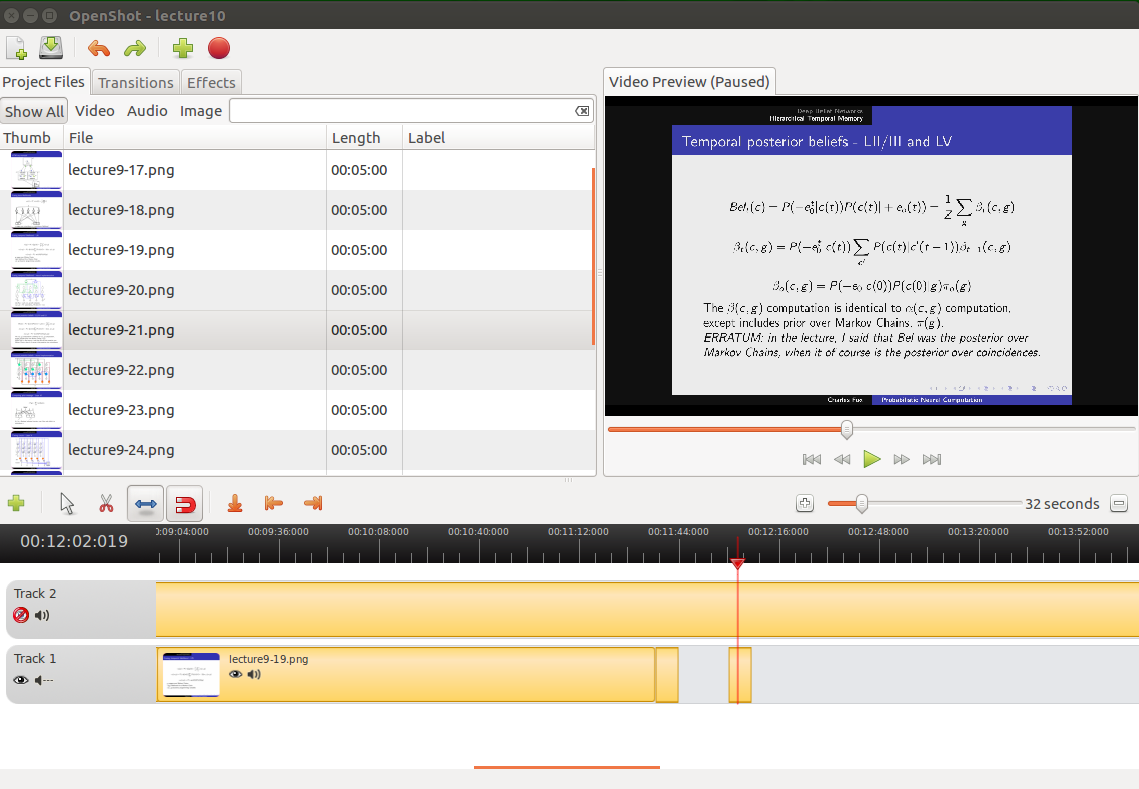
\includegraphics[width=\columnwidth]{figs/openshot.png}
	\caption{OpenShot, used here to edit an audio recording of a lecture together with png-exported Beamer slides.}
  \label{fig:jack-settings}
\end{figure}

Good Linux style is usually to prefer command line tools for basic video editing. For example, see ffpmeg example above for basic commands to cut video files, splice them, and build from or extract still images and audio files.  But for more artistic applications, some users might prefer to use a GUI which wraps these features.

OpenShot allows video, audio, and still-image clips to be combined over time into videos.  It is set up similarly to music software such as Ardour, with tmpora,l tracks show at the bottom of the screen.   At the top left of the screen is the list of available media clips.  

To use OpenShot, first drag each media clip from Nautilus into the set of media clips.  It will appear in the list.  

Then to deploy it in the video track, drag a copy from this list onto the temporal tracks at the bottom.

To crop: select a clip on the temporal track. Then select the resize tool icon just above the temporal track on the left (<--> icon) to resize the two edges.  (Or right clip the clip, go to properties, length to specify with exact numbers.)

To move clips in the temporal track, select the mouse-pointer icon in the abve right.   As in music editors, there are also ways to quantize cut and resize points using a magnet tool, which is on by default and may need to be turned off for fine editing.

OpenShot has tools to add text titles and captions, in its menus.  It also provides various fades and effects (which should be used sparingly to avoid looking like amateur home video).

OpenShot can save the whole project as an OpenShot project file.  It can also export to most major video formats, including preset formats for common applications such as popular Internet video sites.



\section{Desktop screencast recording}

Download the {\em recordmydesktop} tool (e.g. from synaptic). Then just,
\begin{lstlisting}
recordmydesktop
\end{lstlisting}
will record a screencast file, named with the current date and time.  Stop the recording with Ctrl-D.


\section{Zonemaster}
Is a GUI applicatoin for CCTV multi IP-camera control, e.g. for home security monitoring and recording.




\chapter{MISC IDEAS}



(DVD uses H.262/MP2 video;  MP2/MP1/AAC audio, all encrypted)

DVB-T Suite used by digital TV (T for terrestrial, also S for satellite and others)
	codecs:
		video: h.264, AVS ...
		audio: mp3, mp2, aac ...


camera cvlc command , to record
	camea is using http to communicate (?) root/88o88o
	resultion request in cgi URL.  Many settings here too.
	save encode format, currently avi/mpeg, 640x400
	480x360, 20fps.
	as URL, shows CCTV monitor :)

\part{Appendix: Sysadmin for multimedia}

\chapter{Basic sysadmin}

\section{Users}
For laboratory and robotics media systems we will often have a dedicated computer controlling the multimedia hardware.  This computer usually needs to be used my multiple people rather than an individual.   So we set it up to have an abstract user account, here called "ouruser".

Create user account and allow user to use sudo and access USB devices (with are owned by members of the group "dialout"):
\begin{lstlisting}
sudo useradd -m ouruser   #-m to create home directory
sudo passwd ouruser   #give them a password
sudo usermod -aG sudo ouruser
sudo adduser ouruser dialout
\end{lstlisting}

Modify user attributes:
\begin{lstlisting}
usermod -l ouruser ourusernew   #change name (preserve uID)
sudo userdel ouruser   #delete user
groupadd myname
\end{lstlisting}



\section{Setup}

\paragraph{Swapping keys} is often useful.  A lab machine may have unusual form factor and keyboard, or we might just want to make CAPS into ESCAPE to use in vi, or a key might be broken, or we might need a fast way to enter foreign language symbols.

Each hardware key has a numerical code. You need to get the code for the key whose behaviour you want to change.  Obtain a list of all codes by
\begin{lstlisting}
xmodmap -pk
\end{lstlisting}

The seven outputs for each key here are for the key itself, then when pressed with shift, ctrl, Shift+Ctl, AltGr and AltGr+Shift.  (The combinations were once made by extra keys called super,hyper,meta etc.)   To remap the seven outputs for a keycode:

\begin{lstlisting}
xmodmap -e "keycode  60 = period greater a b slash question d"
\end{lstlisting}
(xmodmap can also be given a config file containing many such mappings.  

You may need to remove the 'lock' on each key, then update it, then re-lock it, such as these commands to map Caps Lock to Escape for vi users:

\begin{lstlisting}
xmodmap -e "clear lock"
xmodmap -e "keycode 66 = Escape NoSymbol Escape"
\end{lstlisting}

Add these commands to .bashrc to retain them.


\paragraph{Changing the prompt format} can be very useful for setups where we plan to dial into the machine from outside, in this case it is useful to show the machine name to distinguish from local prompts on the outside machine,
\begin{lstlisting}
\[\e]0;\u@\h: \w\a\]${debian_chroot:+($debian_chroot)}\u@\h:\w\$
\end{lstlisting}

\paragraph{Autologin} is often useful, (xubuntu only?)
\begin{lstlisting}
   /etc/lightdm/lightdm.conf
\end{lstlisting}

\subsection{Ignore laptop lid closures}
Linux when installed on laptops will usually auto-configure to shutdown or sleep when the lid is closed.  If the laptop is indended as use as an unattended media device then we need to either completely disable this behaviour, or in some cases just instruct Linux to turn off the screen but nothing else when the lid is closed.  Usually laptop physical hardware will turn off the screen for us without any action from the OS so we just need to disable all lid close OS behaviours. eg.

        GIU - >  power manager -> do nothing when lid is closed

Or if doesn't work (there are some known GUI bugs): command line version:  edit /etc/systemd/logind.conf to
                        HandlePowerKey=ignore
                        HandleSuspendKey=ignore
                        HandleHibernateKey=ignore
                        HandleLidSwitch=ignore
                


Also we usually need to disable screensavers and automated timer sleepings for lab and robot machine, using whatever desktop GUI is running, or sometimes as config files.

\section{GNU Screen}
Lab and robot machines are usually access remotely via ssh.  A basic ssh connection will kill the whole session if the connection goes down, and only provides one terminal.   Screen solves both problems and provides a persistent session in one or more terminals.

\begin{lstlisting}
sudo apt-get install screen

screen -dRR  #start screen, attach to a session if already exists
screen -ls #list sessions

C-a 0  #go to terminal 0
C-a 1  #go to terminal 1
C-a c  #create new terminal
C-a k  #kill current terminal
C-a K  #kill screen session

\end{lstlisting}

\section{Scheduling automatic program exection times (cron jobs)}

Cron jobs are tasks which are run automatically at given times.  For example taking a picture from a camera every 5 seconds.  ("cron" is a unix program which runs constantly in the background and checks it anything needs to be run from the cron job schedule. "cron" is for "chonometer" or timer.)

to add cron jobs:
\begin{lstlisting}
crontab -e     
\end{lstlisting}
This opens cron config file (cron table) in your favourite editor, for you to add lines describing schedules.  The file MUST end with a return character or will not work!  To add jobs, add lines such as,

\begin{lstlisting}
11 45 * * * touch full/path/to/foo <CR>
\end{lstlisting}
this runs the touch cmd at 11:45 every day.

There is nothing further to do -- cron auto updates everything, and is (usually) always running on linux machines within needing to be turned on.

If a cron job needs to run as root, then add it to root's own chron table rather than your user account's:
\begin{lstlisting}
sudo crontab -e
\end{lstlisting}
(This is particularly useful for rebooting a machine every day to ensure it is in a clean state.)

\section{System logs}

last
shows login history (eg. to check for access by crackers) -- data in /use/adm or similar (a good cracker would remove their logins from this though)

to see reboot history:
$last reboot


\section{USB device naming}

When workng with multimedia we often have USB devices such as cameras, soundcards, and large media storage devices. By default these appear in system with default names like "/dev/sdb1", "/dev/tty1" but it will be convenient, especially if worknig with with robots and other systems that have many devices, to rename them.

The USB protocol ensures that each device knows its own manufacturer name and model name, so the generic Linux USB device driver can see these without any need for other drivers. All other drivers sit on top of the USB drivers and protocols.    Because of this structure, any new USB device can be seen before installing any specific software for it:

\begin{lstlisting}
dmesg
\end{lstlisting}
will show system "device messages" about when devices have been plugged in or removed, which include their model and manufacturer information.

\begin{lstlisting}
ls /dev
\end{lstlisting}
will show all USB devices which act as serial ports in this way. (This is not all devices).

To rename serial devices, we edit the file /etc/udev/rules.d/99-usb-serial.rules to incldude lines which map known manufacturer and model information (eg. obtained from dmesg) to new names:

\begin{lstlisting}
SUBSYSTEM=="tty", ATTRS{idVendor}=="067b", ATTRS{idProduct}=="2303", SYMLINK+="ttyPiksiRadioLink"
SUBSYSTEM=="tty", ATTRS{idVendor}=="067b", ATTRS{idProduct}=="2303", SYMLINK+="ttyGPSgstar"
\end{lstlisting}
Then unplug and replug the device to re-regcnize it as the new name, eg. /dev/ttyPiksiRadioLink . 

If two devices are identical (e.g. two USB cameras used for stereo vision), they can be distinguished by the physical USB port number which they are connected to using the KERNELS attribute describing which physical port they are on (eg 1-4-5 means port 5 of hub on port 4):
\begin{lstlisting}
KERNEL=="ttyUSB*", KERNELS=="1-8.1.5", NAME="ttyUSB0"
KERNEL=="ttyUSB*", KERNELS=="1-8.1.6", NAME="ttyUSB1"
\end{lstlisting}

(See http://askubuntu.com/questions/49910/how-to-distinguish-between-identical-usb-to-serial-adapters#50412 for more details.)


TODO see file notes/usb.txt

TODO devices which are not serial ports, eg webcams.
For devices which are not serial ports but are storage devices, some systems will automatically detect this and mount them in a location such as
/media/

\section{USB mount problems}

On some distributions, security restrictions may prevent access to USB devices by user accounts (eg. for use on shared machines in public places) so access needs to be granted by root, and they will need to be mounted: (TODO check this):

If USB device is blocked due to a previous program still owning it, the error is given, "could not open port dev/tty0 device or resource busy".   To see which process is holding it,
\begin{lstlisting}
fuser /dev/tty0
\end{lstlisting}
Then kill the offending process by its PID number with
\begin{lstlisting}
kill -kill PID
\end{lstlisting}
This works for any file too -- a USB device is just a file and fuser stands for "file user".

Remounting USB devices (assuming user has access, see user setup above),
\begin{lstlisting}
$ sudo umount /dev/sdb1
$ sudo mount -t ntfs -rw /dev/sdb1 hd
\end{lstlisting}

(Some setups have problems with hard discs and USB sticks, if in a rush it can be useful to do transfers as root, eg, 
\begin{lstlisting}
sudo cp foo.pdf /media/usb/document/
\end{lstlisting}
)

\section{Finding data}
Finding text lost in lots of files: this is like running a search engine on the (recursive) contents of a folder (may need to run overnight etc for large data logs etc):
\begin{lstlisting}
find /path/to/search/from/*.{tex,txt,lyx} -type f -print0 | xargs -0 grep -H "phrase to search for"
\end{lstlisting}

\chapter{Local subnets}

[TODO notes/tcpip-myhouse has more, need to separate out]


In experimental labs, on-board robots, grid computing and some studio/office scenarios, we
often want to run a network of devices in a private network which
allows us full control over them.  This gives some security advantages, for example making it harder for an outsider to take control of a robot or camera in our lab; and also reduces the number of IP addresses neede by your organisation. Practically, it means you don't need to ask IT for new IP addresses or tell them about the devices in the lab, because only one gateway machine will be externally visible.

Typically there is a gateway computer
used to operate the devices, and we may wish
it to have LAN/internet access. This document describes how to set up
a local network with Linux machines for these purposes.


\section{Network hardware}

TCP/IP networking has three relevant layers of protocol:

\paragraph{Ethernet} is a low level protcol in which each device on a physical network as a MAC address and can send and receive "frames" (not "packets") of data to another device via its MAC address. MAC addresses are (almost) hardwired into physical network cards. Ethernet is a bus so any frames put on the bus are visible to everyone on the bus.

\paragraph{IP} (Internet protocol) forms and transmits IP packets, over Ethernet, or other media.  It assignes each device an IP address, which is different from the MAC addresses. IP addresses are assigned to machines by software. They can be fixed by local software, or DHCP is a protocol which allows them to be requested from a central server (in order to avoid conflicts and enforce a numbering system).

\paragraph{TCP} is higher level still, and is a protocol which control how IP packets are passed around the (inter)network. Is is the usual way to pass packets.
\paragraph{UDP} is an alternative to TCP, which also controls how IP packets are passed around. It removes most of the error checking and gaurentee of deliverty from TCP so is faster but expects to loose packets. It is used typically for media streaming where low latency is required and there is no point in guarentiing slow deliver of packetes from, say, video frames whose time has already passed.

\paragraph{(ICMP} is a futher protocol for sending error messages such as "host unreachable")

Typically a local network is based around one central switch with
all devices connected directly to it. In some projects, a wifi switch
is also plugged in to enable wifi devices (such as mobile robots)
to connect. A true wifi switch is a different device from a domestic combined
router-hub-modem, though some of these devices can be hacked to function
as switches using open source firmware.

One server machine with two ethernet cards is needed to control traffic
between the local and LAN networks. One card faces the local network and the other faces the public network.  This machine is called the gateway.
As well as routing approrpiate traffic between the two cards, it can be useful to use this machine to host other network services for the local network too, as below.  Often this machine is a dedicated "router" device, as found in "home routers" and also more professional ones; which combines a simple low-power PC with ethernet and wifi cards, a modem, and pre-configured routing, DNS, and DHCP services, usually with some cusotmer-friedly web-based control interface to a subset of their functions. In other cases we can use a regular or rack-server PC to perform the same functions, especially if we want more control over them, as discussed here.

\section{Basic tools}

There are many small differences between distros, and versions of
distros, so use these tools and Google to understand what's going
wrong.

The most essential network status command is,
\begin{lstlisting}
ifconfig
\end{lstlisting}
which in its most basic form (it is capable fo much more) lists all currently active ("up") network cards and their IP and MAC addresses.  If the main card is missing an IP this is an indication something is wrong.  If card not shown in ifconfig, it may be "down" (ie disabled): 
\begin{lstlisting}
ifconfig -a   #list all cards including DOWN 
ifconfig eth1 up    #bring a card back up
\end{lstlisting}

Every time you change anything is is very good practice to restart the network system to ensure the changes take effect, with:

\begin{lstlisting}
service network restart			 #(Ubuntu)
/etc/init.d/networking restart   #(Debian)
/etc/init.d/network restart      #(Fedora)
\end{lstlisting}
It is often useful to do this routinely after nay change to the network to avoid stupid bugs.

This releases our current IP as assigned by a DHCP server, and requests a new one:
\begin{lstlisting}
su
dhclient eth0 -r
dhclient eth0
\end{lstlisting}

Use ping to test if a particular machine is reachable, either by its IP or address,
\begin{lstlisting}
ping 192.168.0.5
ping google.com
\end{lstlisting}

\paragraph{Port scanning} can be performed to list all network devices having ports ssh(22) or http(80) ports open:
\begin{lstlisting}
sudo nmap -sS -p22,80 192.168.1.0/24
sudo nmap -r -sU -p22,53 IP   #UDP scan
\end{lstlisting}
closed means: the port is open, but no app is listening on it

Other useful commands:
\begin{lstlisting}
tracetoute
mtr
ip s r  #show route
ip a r  #add route

arp-scan --interface=p1p1  --localnet    #show who's connected

snoop -packet sniffer tool, monitor traffic between two hosts

netstat - can open ports
netstat -tulpn   #list open ports on server

ps aux #show all processes

dig @192.168.0.1 google.com   #sends a test nslookup to it? , shows chain of nameservers used to find it (need to use a new URL each time to avoid cache)
    (dig is similar to nslookup, personal choice which is best)

nslookup
whois
host
\end{lstlisting}


\section{Removing automated tools}
Ubuntu and other distos sometimes include a user-friendly desktop GUI program which tries to manage networking for us. For example, automatically detecting that an ethernet cable is plugged in or a known wifi network is available, and automatically switching to them.  This is great for consumers but do manage our own networks we will need to remove all of this so that it doens't automatically revert all our changes:

\begin{lstlisting}
remove network-manager (ubuntu,apt-get) NetworkManager(Fedora,yum) package 
\end{lstlisting}
  

\section{Static IP}

IP requires each machine have a software IP address.  In typical offices and homes run a central DHCP server which all other machines contact (via special low level ethernet MAC-based request) and which assigns an IP to each of them.  This is usually a Good Thing because it ensures there is a single central list of mappings from MACs to IPs and no-one will get confused.  

In our own labs, robots etc though, the hassle of running a DHCP server may be too much and Static IPs quicker and easier.  (e.g. if a robot loses its long-range connection to a DHCP server then bad things may happen).   In Static IP, each computer simply has its own file saying what it's own IP address is.  There are no checks to make sure that two computers don't claim the same one - we must ensure this ourselves.  But then we know exactly who is who and don't rely on any other machines.  Computers can simply contact each other via their IPs, such as "ping 192.168.0.5".

define cards here:   (eg which to bring up on boot, which to dhcp on boot, set static IPs?) 
debian              fedora 
\begin{lstlisting}
/etc/network/interfaces     /etc/sysconfig/networking/devices/ifcdf-<cardname>  

debian:
auto eth0
iface eth0 inet dhcp 

iface wlan0 inet static
address 192.168.0.22
netmask 255.255.255.0
gateway 192.168.0.1

fedora: format for static assign is 
UUID="e88f1292-1f87-4576-97aa-bb8b2be34bd3" 
NM_CONTROLLED="yes" 
HWADDR="D8:D3:85:AE:DD:4C" 
BOOTPROTO="static"
DEVICE="em1"
ONBOOT="yes"
IPADDR=192.168.1.2
NETMASK=255.255.255.0
BROADCAST=192.168.1.255
NETWORK=192.168.1.0
GATEWAY=192.168.1.1
    
\end{lstlisting}

should be able to manual assign IPs and ping between them here, using numeric IPs.

\section{Hostnames}

While it is possible to work entirely with numerical IPs, it is convenient to assign a text name to each machine on our local network, these are called hostnames.  Then we can do, for example.
\begin{lstlisting}
ssh myrobot
ping cameraserver1
\end{lstlisting}

For large networks (typically those runnign DHCP) we set all the hostnames centrally, similarly to setting IPs centrally, using a DNS (domain name service) server. This usually runs on the same server machine as DHCP and the gateway.

For small networks, (typically with no DHCP) we just give each indivual machine its own list of mappings from hostnames to IPs, by editing the file,
\begin{lstlisting}
/etc/hosts    #local DNS lookup 
or on some systems,
/etc/hostname   #or use hostname command 
\end{lstlisting}
  

\section{Gateway: routing to the internet}

This section is about how to connect our subnet to a larger network such as a company network or the internet. 

It is important to understand the levels of TCPIP here. A bridge is
an IP-level (Level 2) method of bonding two networks together, meaning that packets
entering one network will also enter the other. Bridging is appropriate
for example between a wifi network and a wired network. Bridging is
not what we want to do to connect our local network to the internet,
because we don't want our internal packets, such as robot control
messages, passing outside the local network. Nor do we want packets
from other uses of the LAN in our office building to circulate in
our local network and interfere with  transmission of high speed data
during an experiment. We want to allow packets from outside to enter
but only if they are destined for one of our machines. The appropriate
level to provide this behaviour is instead the TCP level (level 3), and the method
is routing, not bridging.

IP Masquerading is a system which converts between local and external
IPs. When a machine with local IP 192.168.0.2 requests a web page
from an external machine 123.456.789.123, the packet passes to the
gateway 192.168.0.1, which runs the routing software, in our case
iptables. iptables tests if the packet is addressed to another local
machine or to the outside world. If local, it sends it back out through
the same, local-facing, ethernet card it was received on. If external,
it consumes it, then edits the content of the packet to make it look
as if it was send my its own, external IP, such as 143.222.333.444.
The modified packet is then send out from the other ethernet card,
into the LAN (whose own routers may relay it to the internet.) When
a reply is received, iptables again edits the packets to convert the
target from its own IP to that of the original machine on the local
network, and sends them out on the local network card. iptables is
also a firewall, as it provides many types of control over what kinds
of packets are forwarded in this way and which are discarded.

In practice: on the gateway machine, we can see current card status
with ifconfig. Calling the cards p1p1 and p1p2, we want p1p1 to face
the local network and p1p2 to face the LAN. We can request a global
IP from the LAN's DHCP server by 

\emph{dhclient p2p1}

or by using DHCP's config files to do the same on startup.

We then put the local facing card into ``promiscuous mode'' which
give the system permission to inspect and modify packets send to and
from other machines:

\emph{ifconfig p1p1 promisc}

Next we enable IP forwarding, which allows the gateway to pass packets
between the two cards,

\emph{echo 1 > /proc/sys/net/ipv4/ip\_forward -- temporary setting}

\emph{vi /etc/sysctl.conf ; edit line to set: net.ipv4.ip\_forward
= 1 -- permanent setting}

\emph{sysctl -p /etc/sysctl.conf}

Check that iptables is running,

\emph{service iptables status}

and restart it if any problems,

\emph{service iptables restart}

Then instruct it to perform IP masquerading,

\emph{iptables -A FORWARD -i p2p1 -o p1p1 -m state --state RELATED,ESTABLISHED
-j ACCEPT }

\emph{iptables -A FORWARD -i p1p1 -o p2p1 -j ACCEPT }

\emph{iptables -t nat -A POSTROUTING -o p2p1 -j MASQUERADE}

\emph{Debian: service iptables save Fedora: /usr/libexec/iptables.init
save.}

These commands autoedit the cfile /etc/sysconfig/iptables , can also
be edited by hand.

To accept ssh connections from outside, we need to open the local
ssh port (22), by adding this to the config file:

\emph{-A INPUT -m state --state NEW -m tcp -p tcp --dport 22 -j ACCEPT}

We can check sshd is installed and running with

\emph{service sshd status }

A last step for Fedora/RHEL users. In order for the system to save
the iptables rules we setup we have to configure iptables correctly.
You will need to edit /etc/sysconfig/iptables-config and make sure
IPTABLES\_MODULES\_UNLOAD, IPTABLES\_SAVE\_ON\_STOP, and IPTABLES\_SAVE\_ON\_RESTART
are all set to 'yes'.

Alternatives to iptables include ``Full NAT'' which requires support
from the LAN admins, or use of proxy servers, which requires support
by client machines. Also to use of /etc/hosts.allow and /etc/hosts.deny
on individual machines.

Note iptables is also used by systems like webasr and USTAR to pass
packets received by a public gateway to specific servers depending
on their type.

\section{Routing and firewall: iptables}

 (vs. bridging: (not used, we want a router not a bridge.  brctl    #add bridge, assign cards to it, bring it up)
 (Bridge is L2 ethernet frames and MAC addresses, bonding two networks into one, eg wifi and wired)
 (Router is L3, packets and IPs. Is what we want.)
 (IP-MASQ masquerading is what we want, allow web request from 192.168.0.1 to appear on the inet as router 143 IP. Then rename back by the router (using post numbers in the packet.
   vs. Full NAT, requires subnet  block of addresses from DCS, not allowed
   vs. Proxy server, requires client to know about it and use it, too complex.)
  Routing is done using a firewall, we will use iptables   (vs Ubuntu ufw firewall)

second card: p2p1 connect to internet.   Run DHCP on it, eg
\begin{lstlisting}
dhclient p2p1
\end{lstlisting}
does not conflict with local network -- broadcasts req out to internet, not to local network. Gets IP.
or auto set it to shcp using its interface file.

enter promiscuous mode: (allow iptables etc to see all local net traffic)
ifconfig p1p1 promisc

Enable IP forwarding (ok to pass packets between cards)
\begin{lstlisting}
echo 1 > /proc/sys/net/ipv4/ip_forward      #(cant be saved with vi, must use >) -- temporary setting
vi /etc/sysctl.conf  ;  edit line to set:  net.ipv4.ip_forward = 1    -- permanent setting
sysctl -p /etc/sysctl.conf
\end{lstlisting}

check iptables running:
\begin{lstlisting}
service iptables status             #or restart it, and check /var/log/messages to see it
\end{lstlisting}

\begin{lstlisting}
iptables -A FORWARD -i p2p1 -o p1p1 -m state --state RELATED,ESTABLISHED -j ACCEPT
iptables -A FORWARD -i p1p1 -o p2p1 -j ACCEPT
iptables -t nat -A POSTROUTING -o p2p1 -j MASQUERADE
Debian: service iptables save   #Fedora: /usr/libexec/iptables.init save.
\end{lstlisting}

NB these autoedit the file:  /etc/sysconfig/iptables.   *nat section leave alone, only for NAT stuff.   Main rule section is *filter.
    i might have done the commands int he worng order -- failed until I manually edited the iptables file and moved the host-prohibited lines to the very end before COMMIT.  I think the rules get tried in order, so the prohibs are the fail-through last choice?

to enable ssh accept: open local port 22: add to near top of *filter:   (INPUT is the chain for packets that are delivered to the server itself)
  -A INPUT -m state --state NEW -m tcp -p tcp --dport 22 -j ACCEPT
    service sshd status  #to check its running

Ok last step for Fedora/RHEL users. In order for your system to save the iptables rules we setup in step two you have to configure iptables correctly. You will need to edit /etc/sysconfig/iptables-config and make sure IPTABLES_MODULES_UNLOAD, IPTABLES_SAVE_ON_STOP, and IPTABLES_SAVE_ON_RESTART are all set to 'yes'


\section{DHCP}

The gateway will assign local IPs to local machines via DHCP, but
should not attempt to reply to DHCP requests from the outside LAN.
(The latter would be very, very bad and would lead to a severe telling
off from the IT department.) We must configure DHCP to run only on
the inwards facing card, and tell it what IPs to assign to each machine
(as is done by graphical interfaces in some home routers).

DHCP is provided by the dhcpd deamon, started up with

\emph{service dhcpd restart}

and its main config file is

\emph{/etc/dhcpd/dhcpd.conf}

(location may vary across distros). We edit this file to assign IPs
to the MACs of indiivudal machines on the local network. Before starting
dhcpd, the local facing card must have an IP address, which we assign
using the config file.

To tell dhcpd which cards to operate on, and to avoid the wrath of
IT, we put p1p1 in the file

\emph{/etc/sysconfig/dhcpd}

We will use 192.168.1.0 as the network name, 255.255.255.0 mask (sometimes
written 192.168.1.0/24 where 24 means 24 1's in the mask. (There may
be weird problems with DHCP fails using 192.168.0.0 as the net name,
hence the 1).

The .0 refers to the whole network, not a machine name. The .255 address
is used to broadcast special messages to all machines on the network,
in particular when requesting an IP address from DHCP. By convention,
.254 is often used for routers. 192.168 is a special set of addresses
reserved for local networks, not used as internet addresses.

When testing DHCP, we sometimes want to force a client to request
a new IP, via

\emph{dhcpclient -v -r \#release current IP}

\emph{dhcpclient -v \#request a new one}

\emph{dhcpclient -v eth0 \#request a new one for a specific card,
eg an external IP for the outfacing card.}

Debugging messages from DHCP can be found in

/var/log/messages

(may vary by distro).

To see current leases:

less /var/lib/dhcp/dhclient.leases

\subsection{additional notes - server}

before starting DHCP, p2p1 must have an IP already in the range used in the dhcpd.conf file.  Assign a static one manually.

/etc/sysconfig/dhcpd #lists which card to serve DHCP on (we use p1p1)   *TAKE EXTREME CARE NOT TO SERVE DHCPS TO DCS NETWORK!!!!!!
/etc/dhcp/dhcpd.conf   #lists all machines, ubisensors etc, which subnet to run on.

subnet theory:
    eg use 192.168.1.0 as the network name, 255.255.255.0 mask    (sometimes written 192.168.1.0/24 where 24 means 24 1's in the mask)
    the .0 refers to the whole network, can't name a machine after it as well
    .255 is the broadcast address
    .254 often used for router address, just convention
    192.168 is reseved for local nets, no internet IPs can use it.

weird problems using 192.168.0.0 network, use 192.168.1.0 instead. (DHCP service not starting otherwise)

  debian                fedora  (or use debian way)             fedora-log
/sbin/service dhcpd start       systemctrl restart dhcpd.service    /var/log/messages
/sbin/service dhcpd stop
/sbin/service dhcpd status

debugging: see /var/log/messages for DHCP server output (fedora)
           /var/log/messages   (debian)

\subsection{additional notes - client}

when changing over in 2card mahine:
    double check all physical connections, they often pop out
    sudo dhclient -v -r   #release IP, verbose
    sudo dhclient -v      #request new IP, verbose (useful)
    sudo dhclient -v eth0     #force which card to use (if above doesnt work) (needed on audio PC)

can specify in the interface config files which cards are to req DHCPs on boot.

(i think -v also goes into /var/log/messages ?)



\section{DNS}

We want the local network to do two things with DNS. First, a command
like

\emph{ping google.com}

Should work, by having the gateway machine refer the server name to
a DNS server on the outside LAN.

Second, we would like to name machines inside the local network so
that we can ssh between them more easily.

The linux DNS suite is called bind9 and its main deamon is called
``named'' ("name deamon"). DNS runs as a service on port 53 of the gateway. (Other
useful bind9 tools are the dig debugger and rndc admin tool).

We configure named to be ``authorative'' on internal names, meaning
that it overrules any other DNS servers claiming to know about them,
such as via old caches. Named will also cache external names locally,
but be non-authorative about them if they change.

named settings are made in

\emph{/etc/named.conf}

which on some distros links to included subfiles.

and further settings in

\emph{/var/named/}

By default, named only serves names to its local machine, not the
whole local network. Fix this by enabling it to run on the network
with

\emph{listen-on-port 53 \{127.0.0.1;\}; }

\emph{listen-on-v6-port 53 \{::1;\}; }

\emph{allow-query \{localhost;\};}

And run named with

\emph{service named restart}

Client machines must be instructed who to ask for DNS information,
via 

\emph{/etc/resolve.conf}

then restart their lookup service,

\emph{/etc/init/d/nscd service restart}

Note Ubuntu annoying regenerates this config file with crapware called
resolvconf, remove it before doing this.

Note DNS is a different, more powerful system, than defining /etc/hosts
files on each machine.


\subsection{additoinal notes - DNS}
    we want to have host names like audio-pc.iml assigned by local DNS server, also allow local machines to use google.com etc rather than IPs.
    bind9 is the DNS server suite (as in binding IPs to addresses), its main deamon is called named.  DNS runs on port 53.
        (other parts: dig debugger; rndc admin tool)
    roles: authoritive on (internal) NAT names.   Send out and cache requests for internet names.
        vs. recursive, knows how to call out.   Don't mix the two - instead give clients addresses of both.

    /etc/named.conf
        NB this INCLUDEs other conf files at the end

    systemctrl start named.service      or  service named restart
    log file location - is spec'd in the named.conf (within the "directory" definded, then in "logging")
    see also /var/log/messages on SEVICE STARTUP for errors due to rncd.key ************8

    Fedora: need to change defualt config to allow clients to use named, (defualt, only usable on the sever itself)
        remove these lines from named.conf:  (they restrict use to particular machines)
            listen-on-port 53 {127.0.0.1;};
            listen-on-v6-port 53 {::1;};
            allow-query {localhost;};

    see also files in
        /var/named/

    client machine: /etc/resov.conf tells where to find the dns server  (ubuntu: autogen by resolvconf tool -- spt-get removed it)
        used by service, need to restart when conf changed:
            /etc/init.d/nscd service restart

\section{Mounts}

To mount a remote server,

\emph{sudo sshfs charles@squeal:/share/mini3/data/audvis/usfd/wargames1
wargames1 }

To mount a NAS drive on the local network:

\emph{sudo mount -t nfs 192.168.0.10:/c/recording /home/recorder/ngraid2 }

see \emph{fstab} for permanent mounts -- but careful to have it run
after DHCP and DNS running.

\section{Use}

Once all the above is setup, you can ssh into the gateway machine
using its external IP or name,

\emph{ssh mygateway@mylan.com}

Then from there, ssh into the other local machines,

\emph{ssh mylocalbox3.mylocaldomain}

where the local machine and domain names are defined by DNS. From
your home laptop you can also use your hosts file to give a short
name to the gateway.

\end{document}
